\documentclass[a4paper,openany,12pt]{report}
\usepackage[utf8]{inputenc}
\usepackage{setspace}
\usepackage[romanian]{babel}
\usepackage{amsmath}
\usepackage{amssymb}
\usepackage{amsthm}
\usepackage{latexsym}
\usepackage{graphicx} %Iti permite sa importezi imagini
\usepackage{caption}
\usepackage{float} %Iti permite sa controlezi pozitia
\usepackage{geometry}
\usepackage{coloring}

\newtheorem{theorem}{Teorema}[section]
\newtheorem{definition}{Defini\c tie}[section]
\newtheorem{corollary}{Corolar}[section]
\newtheorem{lemma}{Lema}[section]
\newtheorem{notice}{Observa\c tie}[section]

\newcommand{\R}{\mathbb{R}}
\newcommand{\N}{\mathbb{N}}
\usepackage{exercise}
\renewcommand\AnswerName{Solu\c tie}
\newtheorem{case}{Cazul}

\onehalfspacing
\thispagestyle{empty}


\begin{document}
\begin{center}
	{\large \textbf{UNIVERSITATEA „BABE\c S-BOLYAI” CLUJ-NAPOCA}} \vspace{3mm} %vspace spune cat spatiu lasi in continuare pana la urmatorul rand scris
	
	{\large \textbf{FACULTATEA DE MATEMATIC\u A \c SI INFORMATIC\u A}} \vspace{4cm}

	{\Large \textbf{Lucrare de licen\c t\u a}} \vspace{2cm}

	{\Large \textbf{SERII FOURIER}} \vspace{4cm}
\end{center}
\begin{flushleft}{\large \textbf{Coordonator \c stiin\c tific:\\Conferen\c tiar TRIF Tiberiu}}
\end{flushleft}
\begin{flushright}{\large \textbf{Absolvent:\\ MOLDOVAN Ioana}} \vspace{3cm}
\end{flushright}
\begin{center}
{\large \textbf{2018}}
\end{center}

\newpage
\tableofcontents
\addcontentsline{toc}{chapter}{Introducere}\chapter*{Introducere}
\begin{quote}
„Matematica este un joc care se joac\u a dup\u a anumite reguli simple cu semne f\u ar\u a \^ in\c teles pe h\^ artie.”
\end{quote}
\begin{flushright} David Hilbert
\end{flushright}



Seriile Fourier, denumite astfel \^ in onoarea matematicianului francez, Baptiste Joseph Fourier, sunt un instrument folosit \^ in analiza funcțiilor periodice. Fourier a introdus aceste serii cu scopul de a rezolva ecua\c tia propag\u arii c\u aldurii \^ intr-o plac\u a metalic\u a. Cercet\u arile lui au condus la concluzia c\u a orice func\c tie continu\u a poate fi reprezentat\u a cu ajutorul unei serii trigonometrice. P\^ an\u a la Fourier erau cunoscute doar solu\c tii particulare ale ecua\c tiei c\u aldurii \^ in cazul \^ in care sursa de c\u aldur\u a era dat\u a de o func\c tie periodic\u a de tip sinus sau cosinus. Ideea lui Fourier a fost de a modela surse de c\u aldur\u a de o form\u a mai complicat\u a cu ajutorul unor combina\c tii liniare de func\c tii sinus \c si cosinus.


Cu toate c\u a motiva\c tia lui Fourier a fost rezolvarea ecua\c tiei c\u aldurii, ideile \c si tehnicile lui s-au dovedit ulterior a fi aplicabile \^ in numeroase alte probleme de matematic\u a \c si fizic\u a precum cele din electricitate, acustic\u a, optic\u a, prelucrarea semnalelor, prelucrarea imaginilor, mecanic\u a cuantic\u a.


Lucrarea de fa\c t\u a \^ i\c si propune prezentarea dezvolt\u arii \^ in serie Fourier a unei func\c tii de variabil\u a real\u a, sintetizarea \c si demonstrarea unor teoreme de convergen\c t\u a \c si divergen\c t\u a, precum \c si rezolvarea unor aplica\c tii sugestive cu ajutorul seriilor Fourier. Aceast\u a lucrare este structurat\u a \^ in patru capitole. Primul capitol descrie no\c tiunea de \textit{serie Fourier}, rela\c tiile de ortogonalitate pe care se bazeaz\u a aceasta, accentul fiind pus pe dezvoltarea unei func\c tii reale \^ in serie Fourier. Cel de-al doilea capitol este dedicat enun\c t\u arii \c si demonstr\u arii unor rezultate importante (Teorema 2.3.1, Egalitatea lui Parseval, Criteriul lui Dirichlet) care s\u a precizeze convergen\c ta seriei Fourier a unei func\c tii continue periodice. \^ In paralel cu capitolul precedent, al treilea capitol este menit s\u a eviden\c tieze fenomenele de divergen\c t\u a a seriilor Fourier. \^ In orice caz, ultimul capitol prezint\u a solu\c tiile unor aplica\c tii rezolvate cu ajutorul seriilor Fourier (Aplica\c tii cu referire la conduc\c tia termic\u a, coarda vibrant\u a, ecua\c tia lui Laplace, func\c tia Zeta a lui Riemann). 


Contribu\c tia proprie la realizarea lucr\u arii const\u a \^ in: selectarea \c si structurarea materialului bibliografic, prezentarea mai am\u anun\c tit\u a a unor demonstra\c tii \c si rezolvarea unor aplica\c tii prezentate \^ in ultimul capitol al lucr\u arii (Aplica\c tiile 4.0.6 \c si 4.0.7).



\chapter{Serii Fourier}
\section{Origini}
\paragraph*{}
Seriile Fourier \^ i\c si au r\u ad\u acinile \^ in problemele de fizic\u a matematic\u a, \^ in clasicile probleme de propagare a undelor \c si conduc\c tie termic\u a. Ca exemplu, se consider\u a problema determin\u arii st\u arii de echilibru a distribu\c tiei temperaturii $u(r, \theta)$ \^intr-o plac\u a metalic\u a circular\u a cu raz\u a unitar\u a, d\^ andu-se temperatura de pe frontier\u a $u(1, \theta)=f(\theta)$, unde $r$ \c si $\theta$ sunt coordonatele polare standard. Aici $f$ este considerat\u a o func\c tie arbitrar\u a, nu neap\u arat continu\u a, cu proprieteatea c\u a $f(\theta + 2\pi) = f(\theta)$. \c Tin\^ andu-se seama de legile fizicii, solu\c tia $u(r, \theta)$ va fi o func\c tie armonic\u a, care este solu\c tie a ecua\c tiei lui Laplace. Acesta ia forma urm\u atoare \^ in coordonate polare:
\begin{equation}
\frac{\partial^2 u}{\partial r^2} + \frac{1}{r}\frac{\partial u}{\partial r} + \frac{1}{r^2}\frac{\partial^2 u}{\partial \theta^2} = 0
\end {equation}
\paragraph*{}Dac\u a $f(\theta) = \sin(n\theta)$ sau $\cos(n\theta)$ pentru $n = 1, 2, ...$, aceast\u a problem\u a de determinare a valorii pe frontier\u a poate fi rezolvat\u a prin verificare. Solu\c tiile sunt $u(r, \theta)$ $= r^n \sin(n\theta)$ \c si respectiv $r^n \cos(n\theta)$. Dar ecua\c tia lui Laplace este liniar\u a, a\c sa c\u a se poate aplica principiul superpozi\c tiei. Acest lucru \^ inseamn\u a c\u a pentru orice constant\u a $c$, solu\c tia cu condi\c tia la limita $cf(\theta)$ este $cu(r, \theta)$, iar dac\u a $v(r, \theta)$ este solu\c tia corespunz\u atoare unei alte condi\c tii la limit\u a $g(\theta)$, atunci solu\c tia problemei corespunz\u atoare condi\c tiei la limit\u a $f + g$ este $u + v$.

 
\paragraph*{}Toate acestea sugereaz\u a c\u a problema determin\u arii a valorii pe frontier\u a va fi rezolvat\u a pentru o func\c tie periodic\u a arbitrar\u a $f(\theta)$ dac\u a acea func\c tie poate fi dezvoltat\u a \^ in serie infinit\u a de forma
\begin{equation}
f(\theta) = \frac{a_0}{2} + \sum_{n=1}^{\infty}{\Big(a_n \cos(n\theta) + b_n \sin(n\theta)\Big)}
\end{equation}
pentru coeficien\c tii $a_n$ \c si $b_n$ oarecare. Las\^ and deoparte problema convergen\c tei, se ajunge la solu\c tia:
\begin{equation}
u(r, \theta) = \sum_{n=1}^{\infty}{\Big(a_n r^n \cos(n\theta) + b_n r^n \sin(n\theta)\Big)}.
\end{equation}
\paragraph*{}
O dezvoltare de forma (1.2) se nume\c ste $serie$ $Fourier$.
\paragraph*{}Seriile Fourier au fost denumite dup\u a fizicianul matematician francez Joseph Fourier (1768-1830) care a conceput metoda \c si a dezvoltat-o \^ in importanta sa lucrare despre conduc\c tia termic\u a, $Th\acute{e}orie$ $analytique$ $de$ $la$ $chaleur$ (Teoria analitic\u a a c\u aldurii), publicat\u a \^ in 1822. \^ In particular, era greu de crezut c\u a o func\c tie discontinu\u a poate fi reprezentat\u a ca sum\u a de sinusuri \c si cosinusuri, a\c sa c\u a argumentele lui Fourier au fost privite cu scepticism \c si nu au fost rapid acceptate. Mai t\^ arziu, Cauchy, Dirichlet, Riemann \c si al\c tii au exprimat rezultatele lui Fourier cu mai mare rigurozitate dezvolt\^ and concepte mai precise \^ in analiza matematic\u a.
\paragraph*{}Astfel a ap\u arut o teorie matematic\u a extins\u a a seriilor Fourier cu o larg\u a aplicabilitate, nu numai \^ in fizica matematic\u a, ci \c si \^ in diferite alte domenii precum teoria cod\u arii, transmiterea semnalelor, stocarea \c si recuperarea datelor, cristalografie, imagistic\u a medical\u a \c si matematica pur\u a. Seriile Fourier sunt prototipul pentru o varietate de expansiuni ortogonale care au luat na\c stere \^ in mod similar din problemele de fizic\u a matematic\u a. 


\section{Rela\c tii de ortogonalitate}
\paragraph*{}Seriile Fourier se bazeaz\u a pe rela\c tiile de ortogonalitate pentru func\c tiile sinus \c si cosinus. F\u ac\^ and analogie cu vectorii din spa\c tiul euclidian $\mathbb{R}^n$, spunem c\u a dou\u a func\c tii $f$ \c si $g$ integrabile pe un interval $[a, b]$ sunt $ortogonale$ dac\u a
\begin{equation*}
\int_a^b f(x)g(x)\,dx = 0.
\end{equation*}
\paragraph{} Rela\c tiile fundamentale sunt:
\begin{equation}
\int_{-\pi}^{\pi} \cos(nx)\,dx = \int_{-\pi}^{\pi} \sin(nx)\,dx = 0, 
\end{equation}
pentru $n = 1, 2, ...$ .
\begin{equation}
\int_{-\pi}^{\pi} \cos(nx)\cos(mx)\,dx = \int_{-\pi}^{\pi} \sin(nx)\sin(mx)\,dx = 0, 
\end{equation}
pentru $n, m \in \mathbb{Z}, n \neq m$.
\begin{equation}
\int_{-\pi}^{\pi} \cos(nx)\sin(mx)\,dx = 0,
\end{equation}
pentru $n, m = 1, 2, ...$ .
\begin{equation}
\int_{-\pi}^{\pi} \cos^2(nx)\,dx = \int_{-\pi}^{\pi} \sin^2(nx)\,dx = \pi,
\end{equation}
pentru $n = 1, 2, ...$ .
\paragraph*{}Acestea reies u\c sor din urm\u atoarele identit\u a\c ti trigonometrice:
\begin{enumerate}
	\item $\cos(nx)\cos(mx) = \frac{1}{2} [\cos(n + m)x + \cos(n - m)x],$
	\item $\sin(nx)\sin(mx) = \frac{1}{2} [\cos(n - m)x - \cos(n + m)x],$
	\item $\cos(nx)\sin(mx) = \frac{1}{2} [\sin(n + m)x - \sin(n - m)x],$
	\item $\cos^2(nx) = \frac{1 + cos(2nx)}{2},$ $sin^2(nx) = \frac{1 - cos(2nx)}{2}.$
\end{enumerate}



\section{Defini\c tie}
\paragraph*{}Presupunem c\u a pentru coeficien\c tii $a_k$ \c si $b_k$ oarecare, seria trigonometric\u a
\begin{equation}
f(x) = \frac{a_0}{2} + \sum_{k=1}^\infty \Big(a_k\cos(kx) + b_k\sin(kx)\Big)
\end{equation}
converge uniform pe intervalul $[-\pi, \pi]$ c\u atre o sum\u a $f(x)$. Alegerea termenului liber din seria (1.8) este justificat\u a de motive de simetrie care se vor vedea \^ in continuare.
\paragraph*{}Se \c stie c\u a o serie uniform convergent\u a de func\c tii continue are ca sum\u a o func\c tie continu\u a. Deoarece termenii seriei din rela\c tia (1.8) sunt func\c tii continue, iar seria este uniform convergent\u a, rezult\u a c\u a func\c tia $f$ este continu\u a pe $[-\pi, \pi]$, deci integrabil\u a pe $[-\pi, \pi]$. A\c sadar putem integra termen cu termen rela\c tia (1.8) pe intervalul $[-\pi, \pi]$ \c si ob\c tinem
\begin{equation*}
\int_{-\pi}^\pi f(x)\,dx =\frac{a_0}{2}\int_{-\pi}^\pi \,dx+ \sum_{k=1}^\infty \Bigg(a_k\int_{-\pi}^\pi \cos(kx)\,dx+ b_k\int_{-\pi}^\pi \sin(kx)\,dx\Bigg).
\end{equation*}
\paragraph*{}Conform rela\c tiei (1.4), integralele din paranteza din membrul al doilea sunt egale cu zero, deci ob\c tinem
\begin{equation}
a_0 = \frac{1}{\pi}\int_{-\pi}^\pi f(x)\,dx.
\end{equation}
\paragraph*{}Multiplic\^ and ambii membrii ai rela\c tiei (1.8) cu $\cos(nx)$, ob\c tinem
\begin{equation}
f(x)\cos(nx) = \frac{a_0}{2}\cos(nx) + \sum_{k=1}^\infty \Big(a_k\cos(kx)\cos(nx) + b_k\sin(kx)\cos(nx)\Big).
\end{equation}
\paragraph*{}Deoarece $\cos(nx)$ este o func\c tie m\u arginit\u a, iar seria din rela\c tia (1.8) este uniform convergent\u a, rezult\u a c\u a seria din membrul al doilea al egalit\u a\c tii (1.10) converge uniform pe $[-\pi, \pi]$. Continuitatea produsului $f(x)\cos(nx)$ rezult\u a at\^ at din continuitatea factorilor, c\^ at \c si din faptul c\u a seria uniform convergent\u a din membrul al doilea al rela\c tiei (1.10) are ca termeni func\c tii continue. Pe baza convergen\c tei uniforme putem integra termen cu termen rela\c tia (1.10) \c si ob\c tinem
\begin{equation*}
\int_{-\pi}^\pi f(x)\cos(nx)\,dx = \frac{a_0}{2} \int_{-\pi}^\pi \cos(nx)\,dx + \sum_{k=1}^\infty \Bigg(a_k\int_{-\pi}^\pi \cos(kx)\cos(nx)\,dx +
\end{equation*}
\begin{equation}
 + b_k\int_{-\pi}^\pi \sin(kx)\cos(nx)\,dx\Bigg).
\end{equation}
\paragraph*{}Conform rela\c tiilor de ortogonalitate (1.5), (1.6) \c si (1.7), integralele din membrul al doilea sunt egale cu zero, cu excep\c tia uneia singure, deci ob\c tinem
\begin{equation*}
\int_{-\pi}^\pi f(x)\cos(nx)\,dx = \pi a_n.
\end{equation*}
\paragraph*{}Analog, prin multiplicare cu $\sin(nx)$ se ob\c tine
\begin{equation*}
 \int_{-\pi}^\pi f(x)\sin(nx)\,dx = \pi b_n.
\end{equation*}
\paragraph*{}Numerele
\begin{equation}
 a_n = \frac{1}{\pi}\int_{-\pi}^\pi f(x)\cos(nx)\,dx,\: n = 0, 1, ...
\end{equation}
\begin{equation}
 b_n =\frac{1}{\pi} \int_{-\pi}^\pi f(x)\sin(nx)\,dx, \: n = 1, 2, ...
\end{equation}
se numesc $\textit {coeficien\c tii Fourier ai func\c tiei f}$, iar seria trigonometric\u a din rela\c tia (1.8) este cunoscut\u a ca $\textit {seria Fourier a func\c tiei f}$. Din expresia coeficien\c tilor Fourier observ\u am c\u a ei au sens pentru orice func\c tie integrabil\u a pe $[-\pi, \pi]$, independent de considerarea unei serii trigonometrice. Adic\u a, coeficien\c tii Fourier nu sunt ata\c sa\c ti unei serii trigonometrice, ci unei func\c tii integrabile pe $[-\pi, \pi]$. Oricare ar fi func\c tia $f$ integrabil\u a pe $[-\pi, \pi]$, rela\c tiile (1.12) \c si (1.13) au sens deoarece produsul dintre o func\c tie integrabil\u a \c si o func\c tie continu\u a este o func\c tie integrabil\u a. Deci fiec\u arei func\c tii integrabile pe intervalul $[-\pi, \pi]$ \^ ii corespunde un \c sir infinit de coeficien\c ti Fourier da\c ti de rela\c tiile (1.12) \c si (1.13). Dup\u a cum arat\u a calculele, seria Fourier a unei func\c tii continue $f$ este singura serie trigonometric\u a de forma (1.8) care ar putea converge uniform c\u atre func\c tia $f$ pe $[-\pi, \pi]$. \^ In particular, nici o func\c tie nu are mai mult de o dezvoltare \^ in serie trigonometric\u a uniform convergent\u a. 



\section{Seria Fourier a func\c tiilor pare sau impare}
\paragraph*{} Dac\u a func\c tia $f:[-\pi,\pi]\rightarrow\mathbb{R}$ este par\u a sau impar\u a pe $[-\pi, \pi]$, atunci dezvoltarea ei \^ in serie Fourier se simplific\u a. 
\begin{notice}Dac\u a func\c tia integrabil\u a $f$ definit\u a pe intervalul $[-\pi, \pi]$ este impar\u a, atunci 
\begin{equation*}
\int_{-\pi}^{\pi}f(x)\, dx=0,
\end{equation*} 
iar dac\u a este par\u a, atunci 
\begin{equation*}
\int_{-\pi}^{\pi}f(x)\, dx=2\int_{0}^{\pi}f(x)\, dx.
\end{equation*}
\end{notice}
\paragraph*{}Astfel, dac\u a func\c tia $f(x)$ este \textit{par\u a} pe $[-\pi, \pi]$, atunci func\c tia $f(x)\cos(kx)$ este par\u a, iar func\c tia $f(x)\sin(kx)$ este impar\u a. \c Tin\^ and seama de acestea, vom ob\c tine:
\begin{equation*}
a_0=\frac{1}{\pi}\int_{-\pi}^{\pi}f(x)\, dx =\frac{2}{\pi}\int_0^{\pi}f(x)\, dx,
\end{equation*}
\begin{equation*}
a_k=\frac{1}{\pi}\int_{-\pi}^{\pi}f(x)\cos(kx)\, dx =\frac{2}{\pi}\int_0^{\pi}f(x)\cos(kx)\, dx,
\end{equation*}
\begin{equation*}
b_k=\frac{1}{\pi}\int_{-\pi}^{\pi}f(x)\sin(kx)\, dx = 0.
\end{equation*}
\paragraph*{}A\c sadar, \textit{seria Fourier a unei func\c tii pare con\c tine numai cosinusuri}:
\begin{equation*}
f(x)=\frac{a_0}{2}+\sum_{k=1}^\infty a_k \cos(kx).
\end{equation*}
\paragraph*{}Analog, dac\u a func\c tia $f(x)$ este \textit{impar\u a} pe $[-\pi, \pi]$, atunci func\c tia $f(x)\sin(kx)$ este par\u a, iar  func\c tia $f(x)\cos(kx)$ este impar\u a. Deci vom ob\c tine:
\begin{equation*}
a_0=\frac{1}{\pi}\int_{-\pi}^{\pi}f(x)\, dx =0,
\end{equation*}
\begin{equation*}
a_k=\frac{1}{\pi}\int_{-\pi}^{\pi}f(x)\cos(kx)\, dx =0,
\end{equation*}
\begin{equation*}
b_k=\frac{1}{\pi}\int_{-\pi}^{\pi}f(x)\sin(kx)\, dx = \frac{2}{\pi}\int_0^{\pi}f(x)\sin(kx)\, dx,
\end{equation*}
\paragraph*{}A\c sadar, \textit{seria Fourier a unei func\c tii impare con\c tine numai sinusuri}:
\begin{equation*}
f(x)=\sum_{k=1}^\infty b_k \sin(kx).
\end{equation*}



\section{Dezvoltarea \^ in serie Fourier a func\c tiilor definite pe $[-L, L]$}
\paragraph*{} Teoria construit\u a mai \^ inainte a pornit de la ipoteza c\u a func\c tia dat\u a este definit\u a pentru toate valorile reale ale lui x \c si c\u a este periodic\u a de perioad\u a $2\pi$, \^ ins\u a, vom avea cazuri \^ in care func\c tia periodic\u a dat\u a va fi definit\u a pe un alt interval.
\paragraph*{}Fie $f$ o func\c tie definit\u a pe intervalul arbitrar $[-L,L],\: L>0$, periodic\u a de perioad\u a $2L$ \c si extins\u a pe $\mathbb{R}$ prin condi\c tia de periodicitate $f(x+2L)=f(x)$. Consider\u am func\c tiile $h:\mathbb{R}\rightarrow\mathbb{R},\: g:[-\pi, \pi]\rightarrow\mathbb{R}$ definite prin $h(y)=\frac{yL}{\pi}$ \c si $g(z)=(f\circ h)(z)$, func\c tia $g$ fiind periodic\u a de perioad\u a $2\pi$.
\paragraph*{} Deci avem
\begin{equation*}
g(y+2\pi)=f\big(h(y+2\pi)\big)=f\Big(\frac{y}{\pi}+2L\Big)=f\Big(\frac{yL}{\pi}\Big)=(f\circ h)(t)=g(t), 
\end{equation*}
pentru orice $y\in \mathbb{R}$.
\paragraph*{}Astfel ob\c tinem func\c tia $g$ pentru $y$ \^ in intervalul $[-\pi, \pi]$ la care sunt aplicabile considera\c tiile din subcapitolele precedente. Dac\u a sunt \^ indeplinite anumite condi\c tii, func\c tia poate fi dezvoltat\u a \^ in seria Fourier
\begin{equation*}
g(y)=\frac{a_0}{2}+\sum_{n=1}^\infty\big(a_n\cos(ny)+b_n\sin(ny)\big),\:\text{pentru orice } y\in \mathbb{R},
\end{equation*}
ai c\u arei coeficien\c ti sunt numerele
\begin{equation*}
a_n=\frac{1}{\pi} \int_{-\pi}^{\pi}g(y) \cos(ny)\, dy,\: n=0, 1, ..., 
\end{equation*}
\begin{equation*}
b_n=\frac{1}{\pi} \int_{-\pi}^{\pi}g(y) \sin(ny)\, dy,\: n=1, 2 ...\:.
\end{equation*}
\paragraph*{} Utiliz\^ and substitu\c tia $y=\frac{\pi x}{L}$, ob\c tinem dezvoltarea func\c tiei $f$ \^ in serie Fourier
\begin{equation*}
f(x)=\frac{a_0}{2} + \sum_{n=1}^\infty\bigg(a_n\cos\Big(\frac{n\pi x}{L}\Big)+b_n\sin\Big(\frac{n\pi x}{L}\Big)\bigg),
\end{equation*}
unde
\begin{equation*}
a_n=\frac{1}{L}\int_{-L}^{L} f(x) \cos\Big(\frac{n\pi x}{L}\Big)\, dx,\: n =0, 1, ...,
\end{equation*}
\begin{equation*}
b_n=\frac{1}{L}\int_{-L}^{L} f(x) \sin\Big(\frac{n\pi x}{L}\Big)\, dx, \: n=1, 2, ...,
\end{equation*}
sunt coeficien\c tii acesteia.
\begin{notice}Dac\u a func\c tia $f$ este periodic\u a de perioad\u a $2L$, atunci coeficien\c tii $a_n$ \c si $b_n$ pot fi determina\c ti \c si din formulele echivalente:
\begin{equation*}
a_n=\frac{1}{L}\int_{c}^{c+2L} f(x) \cos\Big(\frac{n\pi x}{L}\Big)\, dx,\: n =0, 1, ...,
\end{equation*}
\begin{equation*}
b_n=\frac{1}{L}\int_{c}^{c+2L} f(x) \sin\Big(\frac{n\pi x}{L}\Big)\, dx, \: n=1, 2, ...,
\end{equation*}
unde $c$ este orice num\u ar real.
\end{notice}






\section{Dezvoltarea \^ in serie Fourier dup\u a cosinusuri sau sinusuri a unei func\c tii definite pe $(0,L)$}
\paragraph*{} Fie $f$ o func\c tie definit\u a pe $[0, L]$. De multe ori este util ca func\c tia $f$ s\u a se dezvolte \^ in serie Fourier dup\u a cosinusuri sau sinusuri. \^ In acest scop, func\c tia cosiderat\u a $f$ se prelunge\c ste pe intervalul $[-L, 0]$ astfel \^ inc\^ at noua func\c tie s\u a fie par\u a sau impar\u a pe intervalul $[-L, L]$.

\paragraph*{}S\u a presupunem c\u a vrem s\u a dezvolt\u am func\c tia $f$ \^ in serie Fourier dup\u a cosinusuri. A\c sadar efectu\u am extinderea par\u a pe intervalul $[-L, 0]$, ob\c tin\^ and astfel o nou\u a func\c tie par\u a $g(x)$ pe intervalul $[-L, L]$:
\begin{equation*}
 g(x) = \left\{ \begin{array}{l l} f(-x), \text{ pentru $x$}\in [-L, 0]\\ f(x),\text{ pentru $x$}\in [0, L]\\ \end{array} \right.
\end{equation*}
\paragraph*{}Dac\u a func\c tia dat\u a $f(x)$ \^ indepline\c ste condi\c tiile lui Dirichlet (Teorema 2.4.1.) pe intervalul $[0, L]$, atunci \c si noua func\c tie $g(x)$ va \^ indeplini aceste condi\c tii pe intervalul $[-L, L]$. Prin urmare, seria Fourier corespunz\u atoare func\c tiei $g$ va fi
\begin{equation}
g(x)=\frac{a_0}{2} +\sum_{n=1}^{\infty}a_n\cos\Big(\frac{n\pi x}{L}\Big), 
\end{equation}
unde
\begin{equation*}
a_0=\frac{1}{L}\int_{-L}^Lg(x)\, dx=\frac{2}{L}\int_0^Lf(x)\, dx,
\end{equation*}
\begin{equation*}
a_n=\frac{1}{L}\int_{-L}^Lg(x)\cos\Big(\frac{n\pi x}{L}\Big)\, dx=\frac{2}{L}\int_0^Lf(x)\cos\Big(\frac{n\pi x}{L}\Big) \, dx,
\end{equation*}
iar $b_n=0$.
\paragraph*{}Deoarece rela\c tia (1.14) are loc \^ in toate punctele de continuitate de pe intervalul $(-L, L)$, \^ in particular va avea loc \c si pe intervalul $(0, L)$. Astfel ob\c tinem dezvoltarea c\u autat\u a numai dup\u a cosinusuri:
\begin{equation*}
f(x)=\frac{a_0}{2} +\sum_{n=1}^{\infty}a_n\cos\Big(\frac{n\pi x}{L}\Big).
\end{equation*}
\paragraph*{}Analog vom proceda \c si pentru a ob\c tine dezvoltarea \^ in serie Fourier dup\u a sinusuri. Efectu\u am o extindere impar\u a a func\c tiei $f$ pe intervalul $[-L, 0]$, \c si astfel vom ob\c tine o nou\u a func\c tie impar\u a pe intervalul $[-L, L]$:
\begin{equation*}
 h(x) = \left\{ \begin{array}{l l} -f(-x), \text{ pentru $x$}\in [-L, 0]\\ f(x),\text{ pentru $x$}\in [0, L]\\ \end{array} \right.
\end{equation*}
\paragraph*{} Dezvoltarea func\c tiei impare $g$ \^ in serie Fourier va fi
 \begin{equation*}
h(x)=\sum_{n=1}^{\infty}b_n\sin\Big(\frac{n\pi x}{L}\Big),
\end{equation*}
unde $a_0=a_n=0$, iar
\begin{equation*}
b_n=\frac{1}{L}\int_{-L}^Lh(x)\sin\Big(\frac{n\pi x}{L}\Big)\, dx=\frac{2}{L}\int_0^Lf(x)\sin\Big(\frac{n\pi x}{L}\Big)\, dx.
\end{equation*}
\paragraph*{}\^ In particular, \^ in orice punct de continuitate din intervalul $[0, L]$ avem urm\u atoarea dezvoltare a func\c tiei $f$ numai dup\u a sinusuri:
\begin{equation*}
f(x)=\sum_{n=1}^{\infty}b_n\sin\Big(\frac{n\pi x}{L}\Big).
\end{equation*}







\chapter{Convergen\c ta seriilor Fourier}
\section{Aproximarea \^ in medie p\u atratic\u a}
\paragraph*{}O \^ intrebare mult mai delicat\u a este dac\u a seria Fourier a unei func\c tii continue periodice va converge punctual sau uniform c\u atre func\c tia $f$. \^ Inainte de a r\u aspunde la aceast\u a \^ intrebare, vom considera problema celei mai bune aproxim\u ari \^ in medie p\u atratic\u a.
\paragraph*{}Consider\u am func\c tia $f$ de p\u atrat integrabil\u a definit\u a pe intervalul $[-\pi, \pi]$ \c si polinoamele trigonometrice de forma
\begin{equation}
T(x) = \frac{c_0}{2} + \sum_{k=1}^n \Big(c_k\cos(kx) + d_k\sin(kx)\Big)
\end{equation}
de grad mai mic sau egal cu n. Ne punem urm\u atoarea \^ intrebare: dintre toate polinoamele trigonometrice $T(x)$, care ne va da cea mai bun\u a aproximare \^ in medie p\u atratic\u a pentru $f$? Cu alte cuvinte, cum ar trebui s\u a alegem coeficien\c tii $c_k$ \c si $d_k$ astfel \^ inc\^ at integrala
\begin{equation}
\int_{-\pi}^{\pi} \Big[f(x) - T(x)\Big]^2\,dx 
\end{equation}
s\u a fie minim\u a? Pentru a r\u aspunde la aceast\u a \^ intrebare vom considera $a_k$ \c si $b_k$ coeficien\c tii Fourier ai func\c tiei $f$ defini\c ti prin rela\c tiile (1.12) \c si (1.13). Rela\c tia (2.2) devine
\begin{equation*}
\int_{-\pi}^{\pi} \Big[f(x) - T(x)\Big]^2\,dx = \int_{-\pi}^{\pi} f^2(x)\,dx - 2\int_{-\pi}^{\pi}f(x)T(x)\, dx + \int_{-\pi}^{\pi}T^2(x)\, dx.
\end{equation*}
\paragraph*{}\c Tin\^ and cont de forma polinomului trigonometric $T(x)$ \c si de dezvoltarea \^ in serie Fourier a lui $f$, ob\c tinem
\begin{equation*}
\int_{-\pi}^{\pi} \Big[f(x) - T(x)\Big]^2\,dx = \int_{-\pi}^{\pi} f^2(x)\,dx - 2\int_{-\pi}^{\pi}\Bigg[\frac{a_0}{2} + \sum_{k=1}^{n}\Big(a_k\cos(kx) + b_k\sin(kx)\Big)\Bigg]\cdot
\end{equation*}
\begin{equation*}\cdot\Bigg[\frac{c_0}{2} + \sum_{k=1}^{n}\Big(c_k\cos(kx) + d_k\sin(kx)\Big)\Bigg]\,dx + \int_{-\pi}^{\pi}\Bigg[\frac{c_0}{2} + \sum_{k=1}^{n}\Big(c_k\cos(kx) + d_k\sin(kx)\Big)\Bigg]^2\,dx.
\end{equation*}
\paragraph*{}Folosind rela\c tiile de ortogonalitate (1.4), (1.6) \c si (1.7), vom ob\c tine
\begin{equation*}
\int_{-\pi}^{\pi} \Big[f(x) - T(x)\Big]^2\,dx = \int_{-\pi}^{\pi} f^2(x)\,dx - \pi a_0 c_0 - 2\pi\sum_{k=1}^{n}(a_kc_k + b_kd_k) + \frac{1}{2}\pi c_0^2 +
\end{equation*}
 \begin{equation}
 + \pi\sum_{k=1}^{n}({c_k^2 + d_k^2}).
\end{equation}
\paragraph*{}Fie 
\begin{equation}
s_n(x) = \frac{a_0}{2} + \sum_{k=1}^n \Big(c_k\cos(kx) + d_k\sin(kx)\Big)
\end{equation}
suma par\c tial\u a de ordin n a seriei Fourier a lui $f$. Aleg\^ and $T(x) = s_n(x)$, ob\c tinem
\begin{equation}
\int_{-\pi}^{\pi} \Big[f(x) - s_n(x)\Big]^2\,dx = \int_{-\pi}^{\pi} f^2(x)\,dx - \frac{1}{2}\pi a_0^2 - \pi \sum_{k=1}^{n}(a_k^2 + b_k^2).
\end{equation}
\paragraph*{}Din (2.5) rezult\u a
\begin{equation}
\int_{-\pi}^{\pi} f^2(x)\,dx = \int_{-\pi}^{\pi} \Big[f(x) - s_n(x)\Big]^2\,dx + \frac{1}{2}\pi a_0^2 + \pi \sum_{k=1}^{n}(a_k^2 + b_k^2).
\end{equation}
\paragraph*{}\^ Inlocuind $\int_{-\pi}^{\pi} f^2(x)\,dx$ din rela\c tia (2.6) \^ in rela\c tia (2.3), ob\c tinem
\begin{equation*}
\int_{-\pi}^{\pi} \Big[f(x) - T(x)\Big]^2\,dx = \int_{-\pi}^{\pi} \Big[f(x) - s_n(x)\Big]^2\,dx + \frac{1}{2}\pi a_0^2 + \pi \sum_{k=1}^{n}(a_k^2 + b_k^2) - \pi a_0 c_0 - 
\end{equation*}
 \begin{equation*}
 - 2\pi\sum_{k=1}^{n}(a_kc_k + b_kd_k) + \frac{1}{2}\pi c_0^2 + \pi\sum_{k=1}^{n}({c_k^2 + d_k^2}).
\end{equation*}
\paragraph*{}Deci
\begin{equation*}
 \int_{-\pi}^{\pi} \Big[f(x) - T(x)\Big]^2\,dx = \int_{-\pi}^{\pi} \Big[f(x) - s_n(x)\Big]^2\,dx + \frac{1}{2}\pi (a_0 - c_0)^2 + \pi\sum_{k=1}^{n}\Big[(a_k - c_k)^2 + (b_k - d_k)^2\Big].
\end{equation*}
\paragraph*{}Deoarece
\begin{equation*}
 \frac{1}{2}\pi (a_0 - c_0)^2 + \pi\sum_{k=1}^{n}\Big[(a_k - c_k)^2 + (b_k - d_k)^2\Big] \geq 0,
\end{equation*}
rezult\u a c\u a
\begin{equation}
 \int_{-\pi}^{\pi} \Big[f(x) - T(x)\Big]^2\,dx\geq \int_{-\pi}^{\pi} \Big[f(x) - s_n(x)\Big]^2\,dx,
\end{equation}
cu egalitate dac\u a $a_0 = c_0$, $a_k = c_k$ \c si $b_k = d_k$ oricare ar fi $k = 1, 2, ...$ .
\paragraph*{}Cu alte cuvinte, polinomul Fourier $s_n$ d\u a cea mai bun\u a aproximare \^ in medie p\u atratic\u a pentru $f$ dintre toate polinoamele trigonometrice cu grad mai mic sau egal cu n.



\section{Inegalitatea lui Bessel. \\Egalitatea lui Parseval}
\paragraph*{}Deoarece 
\begin{equation*}
\int_{-\pi}^{\pi} \Big[f(x) - T(x)\Big]^2\,dx \geq 0,
\end{equation*}
din rela\c tia (2.6) rezult\u a c\u a
\begin{equation*}
\frac{1}{2}\pi a_0^2 + \pi \sum_{k=1}^{n}(a_k^2 + b_k^2) \leq \int_{-\pi}^{\pi} f(x)^2\,dx.
\end{equation*}
\paragraph*{}F\u ac\^ andu-l pe n s\u a tind\u a la infinit, vom vedea c\u a
\begin{equation}
\frac{1}{2}\pi a_0^2 + \pi \sum_{k=1}^{\infty}(a_k^2 + b_k^2) \leq \int_{-\pi}^{\pi} f(x)^2\,dx.
\end{equation}
\paragraph*{}Rela\c tia (2.8) este cunoscut\u a sub numele de \textit{Inegalitatea lui Bessel}. Aceas\u a inegalitate este valabil\u a pentru sisteme mai generale de func\c tii ortogonale pentru c\u a nu au fost folosite propriet\u a\c ti speciale ale func\c tiilor sinus \c si cosinus \^ in ob\c tinerea ei.
\paragraph*{} Pentru sistemul trigonometric considerat putem afirma c\u a
\begin{equation}
\frac{1}{2}\pi a_0^2 + \pi \sum_{k=1}^{\infty}(a_k^2 + b_k^2) = \int_{-\pi}^{\pi} f(x)^2\,dx.
\end{equation}
\paragraph*{} Identitatea (2.9) este cunoscut\u a sub numele de \textit{Egalitatea lui Parseval}. Aceasta va rezulta din rela\c tia (2.5) dac\u a vom putea ar\u ata c\u a
\begin{equation}
\lim_{n\to \infty} {\int_{-\pi}^{\pi} \Big[f(x) - s_n(x)\Big]^2\,dx} = 0.
\end{equation}
\paragraph*{}Pentru a putea demonstra acest lucru vom apela la forma trigonometric\u a a teoremei de aproximare a lui Weierstrass.
\begin{theorem} [Teorema de aproximare a lui Weierstrass]
Fie $f$ o func\c tie continu\u a pe intervalul $[-\pi, \pi]$ cu proprietatea c\u a $f(-\pi) = f(\pi)$. Atunci oricare ar fi $\varepsilon > 0$, exist\u a un polinom trigonometric astfel \^ inc\^ at $\left | f(x) - T(x) \right | < \varepsilon$, pentru orice x din intervalul $[-\pi, \pi]$.
\end{theorem}
\paragraph*{}Din teorema de densitate a func\c tiilor continue \^ in $L_2[-\pi, \pi]$, rezult\u a c\u a oricare ar fi $ \varepsilon_1 > 0, $ exist\u a o func\c tie $g : [-\pi, \pi] \rightarrow \mathbb{R}$ continu\u a, cu proprietatea c\u a $g(-\pi) = g(\pi)$ astfel \^ inc\^ at
\begin{equation*}
\|f(x) - g(x)\|_{L_2[-\pi, \pi]} < \varepsilon_1, \: \text{oricare ar fi } x \in [-\pi, \pi].
\end{equation*}
\paragraph*{}Aplic\^ and lui $g$ forma trigonometric\u a a teoremei de aproximare a lui Weierstrass, ob\c tinem c\u a oricare ar fi $ \varepsilon_2 > 0,$ exist\u a $T$ un polinom trigonometric astfel \^ inc\^ at  $\left | g(x) - T(x) \right | < \varepsilon_2$, pentru orice x $\in [-\pi, \pi]$.
\paragraph*{}Deci avem c\u a
\begin{equation}
\int_{-\pi}^{\pi} \Big[g(x) - T(x)\Big]^2\,dx < \int_{-\pi}^{\pi} \varepsilon_2^2\, dx.
\end{equation}
\paragraph*{} Aleg\^ and $\varepsilon_1 = \frac{\sqrt \varepsilon}{2}$ \c si $\varepsilon_2 = \frac{\sqrt \varepsilon}{2\sqrt{2\pi}}$, vom ob\c tine
\begin{equation}
\|f(x) - g(x)\|_{L_2[-\pi, \pi]} <  \frac{\sqrt \varepsilon}{2},\: \text{oricare ar fi } x \in [-\pi, \pi]
\end {equation}
\begin{equation}
\left | g(x) - T(x) \right | <  \frac{\sqrt \varepsilon}{2\sqrt{2\pi}},\: \text{oricare ar fi } x \in [-\pi, \pi].
\end {equation}
\paragraph*{} \c Tin\^ and cont de rela\c tia (2.13), rela\c tia (2.11) devine
\begin{equation*}
\int_{-\pi}^{\pi} \Big[g(x) - T(x)\Big]^2\,dx < \int_{-\pi}^{\pi} {\frac{\sqrt \varepsilon}{2\sqrt{2\pi}}}^2\, dx = \frac{\varepsilon}{4}. 
\end{equation*}
\paragraph*{}Rezult\u a
\begin{equation*}
\sqrt{\int_{-\pi}^{\pi} \Big[g(x) - T(x)\Big]^2\,dx } = \|g(x) - T(x)\|_{L_2[-\pi, \pi]}^2 < \sqrt{\frac{\varepsilon}{4}} = \frac{\sqrt \varepsilon}{2}.
\end{equation*}
\paragraph*{}Deci
\begin{equation}
\|g(x) - T(x)\|_{L_2[-\pi, \pi]} < \frac{\sqrt \varepsilon}{2}, \: \text{oricare ar fi } x \in [-\pi, \pi].
\end{equation}
\paragraph*{} Deoarece
\begin{equation*}
\|f(x) - T(x)\|_{L_2[-\pi, \pi]} < \|f(x) - g(x)\|_{L_2[-\pi, \pi]} + \|g(x) - T(x)\|_{L_2[-\pi, \pi]},
\end{equation*}
atunci \c tin\^ and cont de rela\c tiile (2.12) \c si (2.14), ob\c tinem
\begin{equation*}
\|f(x) - T(x)\|_{L_2[-\pi, \pi]} < \frac{\sqrt \varepsilon}{2} + \frac{\sqrt \varepsilon}{2} = \sqrt \varepsilon,\: \text{oricare ar fi } x \in [-\pi, \pi].
\end{equation*}
\paragraph*{} Deci
\begin{equation}
 \int_{-\pi}^{\pi} \Big[f(x) - T(x)\Big]^2\,dx < {\sqrt \varepsilon}^2 = \varepsilon,\: \text{oricare ar fi } x \in [-\pi, \pi].
\end{equation}
\paragraph*{} \^ In subcapitolul precedent am v\u azut c\u a polinomul Fourier $s_n$ d\u a cea mai bun\u a aproximare \^ in medie p\u atratic\u a pentru $f$ dintre toate polinoamele trigonometrice de grad cel mult n. Dac\u a $T$ are gradul m, atunci $\: \text{oricare ar fi }$ n $\geq$ m, avem c\u a
\begin{equation*}
\int_{-\pi}^{\pi} \Big[f(x) - s_n(x)\Big]^2\,dx \leq \int_{-\pi}^{\pi} \Big[f(x) - T(x)\Big]^2\,dx.
\end{equation*}
\paragraph*{}Conform rela\c tiei (2.15) avem c\u a
\begin{equation*}
\int_{-\pi}^{\pi} \Big[f(x) - s_n(x)\Big]^2\,dx < \varepsilon.
\end{equation*}
\paragraph*{} Trac\^ and la limit\u a, ob\c tinem c\u a (2.10) are loc, deci egalitatea lui Parseval este demonstrat\u a. 



\section{Convergen\c ta punctual\u a}
\paragraph*{}Scopul nostru este de a determina condi\c tii care s\u a ne asigure faptul c\u a seria Fourier asociat\u a unei func\c tii $f$ converge c\u atre aceasta. Pentru a ob\c tine o form\u a convenabil\u a a sumei par\c tiale, vom \^ incepe cu un calcul elementar. 
\begin{lemma}Pentru orice $x \in \mathbb{R}\setminus \{2k\pi \mid k \in \mathbb{Z}\}$ \c si orice $n \in \mathbb{N}$ are loc egalitatea
\begin{equation}
\frac{1}{2} + \sum_{k=1}^{n}\cos(kx) = \frac{\sin\Big(x\big(n + \frac{1}{2}\big)\Big)}{2\sin\Big(\frac{1}{2}x\Big)}.
\end{equation}
\end{lemma}
\begin{proof} 
Multiplic\^ and rela\c tia (2.16) cu $2\sin(\frac{1}{2}x)$, aceasta va fi echivalent\u a cu
\begin{equation}
\sin\Big(\frac{1}{2}x\Big) + \sum_{k=1}^n 2\sin\Big(\frac{1}{2}x\Big)\cos(kx)  = \sin\Big(x\Big(n + \frac{1}{2}\Big)\Big).
\end{equation}
Vom folosi urm\u atoarea identitate:
\begin{equation*}
\sin\Big(\frac{1}{2}x\Big)\cos(kx) = \frac{1}{2}\Big[\sin\Big(\Big(k + \frac{1}{2}\Big)x\Big) - \sin\Big(\Big(k - \frac{1}{2}\Big)x\Big)\Big) \Big].
\end{equation*}
Deci rela\c tia (2.17) va fi echivalent\u a cu
\begin{equation*}
\sin\Big(\frac{1}{2}x\Big) + \sum_{k=1}^{n}{\Big[\sin\Big(\Big(k + \frac{1}{2}\Big)x\Big) - \sin\Big(\Big(k - \frac{1}{2}\Big)x\Big)\Big) \Big]}. 
\end{equation*}
Deci ob\c tinem
\begin{equation*}
\sin\Big(\frac{1}{2}x\Big) + \sin\Big(\Big(1+\frac{1}{2}\Big)x\Big) - \sin\Big(\Big(1-\frac{1}{2}\Big)x\Big)  + \sin\Big(\Big(2+\frac{1}{2}\Big)x\Big) -\sin\Big(\Big(2-\frac{1}{2}\Big)x\Big) + ... 
\end{equation*}
\begin{equation}
+\sin\Big(\Big(n+\frac{1}{2}\Big)x\Big)  - \sin\Big(\Big(n-\frac{1}{2}\Big)x\Big)  = \sin\Big(\Big(n+\frac{1}{2}\Big)x\Big).
\end{equation}
Termenii din membrul st\^ ang al rela\c tiei (2.18) se vor reduce \^ intre ei, astfel lema este demonstrat\u a.
\end{proof}
\paragraph*{}Func\c tia 
\begin{equation*}
D_n(x) =  \frac{\sin\Big(x\big(n + \frac{1}{2}\big)\Big)}{2\sin\big(\frac{1}{2}x\big)},\: n=1, 2, ...
\end{equation*}
este cunoscut\u a sub numele de \textit{nucleul lui Dirichlet}. \c Tin\^ andu-se cont de Lema 2.3.1 \c si de faptul c\u a
\begin{equation*} \int_{-\pi}^{\pi}\cos(kx)\, dx = 0,\:\text{pentru }k=1, 2, ..., 
\end{equation*}
func\c tia aceasta are urm\u atoarea proprietate:
\begin{equation}
\frac{1}{\pi}\int_{-\pi}^{\pi} D_n(x)\, dx = 1,\: n = 1, 2, ...\text{ .} 
\end{equation}
\paragraph*{}Nucleul lui Dirichlet este o func\c tie par\u a, periodic\u a de perioad\u a $2\pi.$ Adic\u a
\begin{equation*}
D_n(-x) = D_n(x) \text{ \c si } D_n(x+2\pi) = D_n(x),\:\text{oricare ar fi } x \in [-\pi, \pi].
\end{equation*}
\paragraph*{}Cu ajutorul Lemei 2.3.1 putem determina o form\u a util\u a pentru suma par\c tial\u a de ordin n a seriei Fourier a func\c tiei $f$ definit\u a prin rela\c tia (2.4). 
\paragraph*{}Fie $f$ o func\c tie integrabil\u a pe intervalul $[-\pi, \pi]$ cu prorpietatea c\u a $f(-\pi) = f(\pi)$ pe care o vom extinde pe $\mathbb{R}$ prin periodicitate de perioad\u a $2\pi$. \c Tin\^ and cont de rela\c tiile (1.9), (1.12) \c si (1.13), putem scrie
\begin{equation*}
s_n(x) = \frac{1}{2\pi}\int_{-\pi}^{\pi}f(t)\,dt+ \sum_{k=1}^{n}\frac{1}{\pi}\int_{-\pi}^{\pi}[\cos(kx)\cos(kt)+\sin(kx)\sin(kt)]f(t)\, dt = 
\end{equation*}
\begin{equation*}
= \frac{1}{\pi}\int_{-\pi}^{\pi}\bigg[\frac{1}{2} + \sum_{k=1}^{n}\big( \cos(kx)\cos(kt)+\sin(kx)\sin(kt)\big)\bigg]f(t)\, dt 
\end{equation*}
\paragraph*{}Deci rezult\u a
\begin{equation}
s_n(x) = \frac{1}{\pi}\int_{-\pi}^{\pi}\bigg[\frac{1}{2} + \sum_{k=1}^{n}\cos\big(k(x-t)\big)\bigg]f(t)\, dt.
\end{equation}
\paragraph*{}\c Stiind c\u a
\begin{equation*}D_n(x) = \frac{\sin\Big(x\big(n + \frac{1}{2}\big)\Big)}{2\sin\big(\frac{x}{2}\big)} = \frac{1}{2} + \sum_{k=1}^{n}\cos(kx),
\end{equation*}
egalitatea din rela\c tia (2.20) devine
\begin{equation}
s_n(x) =\frac{1}{\pi} \int_{-\pi}^{\pi} D_n(x-t) f(t)\, dt.
\end{equation}
\c Tin\^ and cont de faptul c\u a $D_n$ este func\c tie par\u a \c si c\u a at\^ at $D_n$, c\^ at \c si $f$ sunt func\c tii periodice de perioad\u a $2\pi$, rela\c tia (2.21) devine
\begin{equation*}
s_n(x) =\frac{1}{\pi} \int_{-\pi}^{\pi} D_n(x-x-t) f(x+t)\, dt = \frac{1}{\pi} \int_{-\pi}^{\pi} D_n(t) f(x+t)\, dt.
\end{equation*}
\paragraph*{}
Rela\c tia
\begin{equation*}
s_n(x) =  \frac{1}{\pi} \int_{-\pi}^{\pi} D_n(t) f(x+t)\, dt
\end{equation*}
este cunoscut\u a sub numele de \textit{formula lui Dirichlet pentru suma par\c tial\u a de ordin n a seriilor Fourier}.
\paragraph*{}Avem
\begin{equation*}
s_n(x) =  \frac{1}{\pi} \int_{-\pi}^{\pi} D_n(t) \big[f(x+t) -f(x) + f(x)\big]\, dt = 
\end{equation*}
\begin{equation*}
= \frac{1}{\pi} \int_{-\pi}^{\pi} D_n(t) \big[f(x+t) -f(x)\big]\, dt + \frac{1}{\pi} \int_{-\pi}^{\pi} D_n(t) f(x)\, dt
\end{equation*}.
\paragraph*{}\c Tin\^ and cont de rela\c tia (2.19), ob\c tinem
\begin{equation}
s_n(x) - f(x) = \frac{1}{\pi} \int_{-\pi}^{\pi} D_n(t) \big[f(x+t) -f(x)\big]\, dt .
\end{equation}
\paragraph*{}Pentru a ar\u ata c\u a $s_n(x) \text{ tinde c\u atre } f(x)$ c\^ and n$\text{ tinde la }  \infty$, trebuie s\u a demonstr\u am c\u a membrul drept al rela\c tiei (2.22) tinde c\u atre zero. Din p\u acate, este posibil ca seria Fourier a unei func\c tii continue periodice s\u a fie divergent\u a \^ in anumite puncte (principiul condens\u arii singularit\u a\c tilor). Pentru a demonstra c\u a seria Fourier converge c\u atre func\c tie \^ intr-un punct dat, ar trebui s\u a impunem ipoteze mai puternice dec\^ at continuitatea. Vom considera c\u a func\c tia satisface o condi\c tie mai fin\u a \^ in vecin\u atatea punctului \^ in care se studiaz\u a convergen\c ta. Formularea precis\u a de netezime este urm\u atoarea:
\begin{theorem}[Teorema de convergen\c t\u a]
Fie $f$ o func\c tie de p\u atrat integrabil\u a pe intervalul $[-\pi, \pi]$ \c si fie $s_n$ suma par\c tial\u a de ordin n a seriei Fourier a func\c tiei $f$. Fie f extins\u a pe axa real\u a prin condi\c tia de periodicitate $f(x+2\pi)=f(x)$. Presupunem c\u a \^intr-un punct $x \in \mathbb{R}$ prelungirea func\c tiei satisface urm\u atoarea condi\c tie de tip Lipschitz:
\begin{equation*}
\left| f(x+t)-f(x) \right| \leq C\left|t\right|, \:\left|t\right|<\delta
\end{equation*}
unde $C$ \c si $\delta$ sunt constante independente de $x$. 
Atunci $s_n(x) \text{ tinde c\u atre } f(x)$ c\^ and n$\text{ tinde la }  \infty$.
\end{theorem}
\paragraph*{}\^ Inainte de a \^ incepe demonstra\c tia, s\u a observ\u am o consecin\c t\u a remarcabil\u a a acestei teoreme. Coeficien\c tii Fourier $a_k$ \c si $b_k$ sunt determina\c ti de valoarea func\c tiei $f$ pe un interval de lungime $2\pi$, totu\c si convergen\c ta seriei Fourier rezultate \^ intr-un punct fixat $x$ este guvernat\u a numai de comportamentul func\c tiei $f$ \^ intr-o vecin\u atate arbitrar\u a a lui $x$. Acest fenomen este cunoscut sub numele de \textit{principiul de localizare al lui Riemann}.
\begin{proof}
%\begin{align*}
%\intertext{}
Corolarul inegalit\u a\c tii lui Bessel privind coeficien\c tii Fourier ai unei func\c tii de p\u atrat integrabile $g$ ne spune c\u a ace\c stia tind c\u atre 0 c\^ and n tinde c\u atre $\infty$. Astfel avem:
\begin{equation}
\lim_{n\to\infty}\int_{-\pi}^{\pi}g(t) \cos(nt)\, dt = \lim_{n\to\infty}\int_{-\pi}^{\pi}g(t) \sin(nt)\, dt = 0. 
\end{equation}
Vom scrie rela\c tia (2.22) \^ in felul urm\u ator:
\begin{equation*}
s_n(x) - f(x) = \frac{1}{\pi} \int_{-\pi}^{\pi}\frac{\sin\Big(x\big(n + \frac{1}{2}\big)\Big)}{2\sin\big(\frac{x}{2}\big)} [f(x+t)-f(t)]\,dt =
%\tag{3} \\
\end{equation*}
\begin{equation*}
= \frac{1}{\pi}\int_{-\pi}^{\pi}\varphi_x(t) \sin\Big(t\Big(\frac{1}{2}+n\Big)\Big)\, dt,
%\end{align*}
\end{equation*}
unde
\begin{equation*}
\varphi_x(t) = \frac{f(x+t)-f(t)}{2\sin\big(\frac{t}{2}\big)}.
\end{equation*}
Pe baza ipotezei lui $f$, vom avea
\begin{equation*}
\left| \varphi_x(t) \right| = \frac{\left| f(x+t)-f(t) \right|}{2\left|sin\big(\frac{t}{2}\big)\right|} \leq \frac{C(t)}{\left|sin\big(\frac{1}{2}t\big)\right|},\: \text{pentru} \: \left|t\right|\leq\delta.
\end{equation*}
Deoarece $\left|\sin\big(\frac{t}{2}\big)\right| \leq 1$, vom ob\c tine c\u a $\left| \varphi_x(t)\right| \leq C$, pentru $\left|t\right|\leq\delta$. Pe de alt\u a parte, dac\u a $t \in[\-\pi, \pi]$ \c si $\left|t\right|>\delta$, atunci avem
\begin{equation*}
\left|\sin\Big(\frac{t}{2}\Big)\right| = \sin \frac{\left|t\right|}{2} > \sin\frac{\delta}{2}=\sin \left|\frac{\delta}{2}\right| > 0.
\end{equation*}
A\c sadar func\c tia $\varphi_x(t)$ este de p\u atrat integrabil\u a pe intervalul $[-\pi, \pi]$. \c Stiind c\u a
\begin{equation*}
\sin\Big(\Big(\frac{1}{2}+n\Big)n\Big) = \sin(nt)\cos\Big(\frac{1}{2}t\Big) + \sin\Big(\frac{1}{2}t\Big)\cos(nt), 
\end{equation*}
avem c\u a
\begin{equation*}
s_n(x) - f(x) = \frac{1}{\pi} \int_{-\pi}^{\pi} \varphi_x(t)\Big[ \sin(nt)\cos\Big(\frac{1}{2}t\Big) + \sin\Big(\frac{1}{2}t\Big)\cos(nt)\Big]\,dt.
\end{equation*}
Rezult\u a
\begin{equation*}
s_n(x) - f(x) = \frac{1}{\pi} \int_{-\pi}^{\pi} \varphi_x(t)\cos\Big(\frac{1}{2}t\Big) \sin(nt)\,dt +
\end{equation*}
\begin{equation}
+ \frac{1}{\pi} \int_{-\pi}^{\pi} \varphi_x(t) \sin\Big(\frac{1}{2}t\Big)\cos(nt)\Big]\,dt.
\end{equation}
Deci integrala din rela\c tia (2.24) poate fi privit\u a ca sum\u a de coeficien\c ti Fourier ai func\c tiilor de p\u atrat integrabile $\varphi_x(t)\cos\Big(\frac{1}{2}t\Big)$ \c si $\varphi_x(t) \sin\Big(\frac{1}{2}t\Big)$. \c Tin\^ and cont de corolarul inegalit\u a\c tii lui Bessel (2.23), avem c\u a integralele din rela\c tia (2.24) tind c\u atre 0 c\^ and n tinde la infinit. Deci $s_n(x) \text{ tinde c\u atre } f(x), \text{ oricare ar fi } x \text{ din } [-\pi, \pi],$ c\^ and n $\text{tinde la } \infty$, adic\u a $\displaystyle{\lim_{n\to\infty} }{s_n(x)} = f(x)$, $\: \text{oricare ar fi } x\in[-\pi, \pi]$.
\end{proof}



\section{Criteriul lui Dirichlet}
\begin{definition} Fie $f:D\rightarrow\mathbb{R}, \: D\subset\mathbb{R},$ o func\c tie \c si $x_0\in\overline{\mathbb{R}}$ un punct de acumulare al mul\c timii $D$. Not\u am
\begin{equation*}
f(x_0-0) = \lim_{x\nearrow x_0}f(x)
\end{equation*}
limita la st\^ anga a func\c tiei $f$ \^ in punctul $x_0$ \c si
\begin{equation*}
f(x_0+0) = \lim_{x\searrow x_0}f(x)
\end{equation*}
limita la dreapta a func\c tiei $f$ \^ in punctul $x_0$, \^ in ipoteza c\u a ambele limite exist\u a.
\end{definition}

\begin{theorem}[Criteriul lui Dirichlet]
Fie $f:\mathbb{R}\rightarrow \mathbb{R}$ o func\c tie periodic\u a de perioad\u a $2\pi$, continu\u a (cu excep\c tia eventual a unui num\u ar finit de puncte de dis-continuitate de prima spe\c t\u a) \c si monoton\u a pe por\c tiuni pe intervalul $[-\pi, \pi]$. Atunci seria Fourier asociat\u a acestei func\c tii, 
\begin{equation*}
\frac{a_0}{2} + \sum_{n=1}^\infty \Big(a_n\cos(nx) + b_n\sin(nx)\Big),
\end{equation*} 
este convergent\u a \^ in toate punctele \c si suma ei este:
\begin{enumerate}
\item $f(x)$, \^ in fiecare punct de continuitate $x$;
\item $\frac{f(x+0)-f(x-0)}{2}$, dac\u a $x$ este punct de discontinuitate pentru $f$.
\end{enumerate}
\end{theorem}
\begin{notice} Condi\c tiile din Teorema 2.4.1 sunt cunoscute sub numele de \textit{condi\c tiile lui Dirichlet}.
\end{notice}
\begin{notice} Teorema 2.4.1 are loc \c si pentru func\c tii de perioad\u a $2L$, $L>0$.
\end{notice}



\chapter{Divergen\c ta seriilor Fourier}
\section{Principul condens\u arii singularit\u a\c tilor}
\paragraph*{}\^ In paralel cu cercet\u arile din secolul al XIX-lea menite s\u a fundamenteze procedeele clasice de aproximare (interpolarea Lagrange, dezvoltarea \^ in serie Fourier, formulele de cuadratur\u a) s-au eviden\c tiat \c si fenomene de divergen\c t\u a a acestor procedee pentru anumite func\c tii, numite ast\u azi \textit{func\c tii singulare }sau \textit{puncte singulare}. Ap\u arut ca o sintez\u a a cercet\u arilor men\c tionate, \textit{principiul condens\u arii singularit\u a\c tilor} precizeaz\u a prin termenul de $superdensitate$, cardinalitatea \c si structura topologic\u a a mul\c timiilor punctelor singulare specifice acestor procedee de aproximare. 
\paragraph*{}
Fie $X$ \c si $ Y$ dou\u a spa\c tii normate \c si $\mathcal{A} \subset Y^X$ o familie de aplica\c tii de la $X$ la $Y$. Vrem s\u a cercet\u am structura mul\c timii
\begin{equation*}
S_{\mathcal{A}} = \big\{x \in X \mid \sup\{\|A(x)\| \mid A \in \mathcal{A}\} = \infty\big\}
\end{equation*}
numite \textit{mul\c timea singularit\u a\c tilor lui A}. \^ In acest scop, introducem urm\u atoarele defini\c tii:
\begin{definition} O submul\c time $Y$ a unui spa\c tiu topologic $X$ se nume\c ste:
\begin{itemize}
\item $\textbf{dens\u a}$ \^ in $X$ dac\u a aderen\c ta lui $Y$ este egal\u a cu $X$.
\item $\textbf{rar\u a}$ \^ in $X$ dac\u a are interiorul vid.
\item $\textbf{num\u arabil\u a}$ \^ in $X$ dac\u a $Y \sim \mathbb{N}$, adic\u a dac\u a $Y$ \c si $\mathbb{N}$ au acela\c si cardinal.
\item $\textbf{de cateoria \^ int\^ ai}$ \^ in $X$ dac\u a exist\u a o familie num\u arabil\u a $\{Y_n \mid n \in \mathbb{N}\}$ de submul\c timi rare $Y_n$ ale lui $X$, cu $Y = \cup \:\{Y_n \mid n \in \mathbb{N}\}$.
\item $\textbf{rezidual\u a}$ \^ in $X$ dac\u a $Y$ este complementara unei mul\c timi de categoria \^ int\^ai \^ in $X$.
\end{itemize}
\end{definition}
\begin{definition}
O submul\c time $S$ a unui spa\c tiu topologic $T$ se nume\c ste $\textbf{superdens\u a}$ \^ in $T$ dac\u a $S$ este dens\u a, nenum\u arabil\u a \c si rezidual\u a \^ in $T$.
\end{definition}

\begin{theorem}[Princiupiul condens\u arii singularit\u a\c tilor]
Fie $X$ \c si $Y$ dou\u a spa\c tii normate pe acela\c si $K$ \c si $\mathcal{A} \subset (X, Y)^*$. Dac\u a $X$ este complet \c si dac\u a 
\begin{equation*}
\sup\{\|A(x)\| \mid A \in \mathcal{A}\} = \infty,
\end{equation*}atunci mul\c timea $S_{\mathcal{A}}$ a singularit\u a\c tilor lui A este superdens\u a \^ in $X$.
\end{theorem}
\begin{proof}
Not\^ and
\begin{equation}
X_n = \cup\: \big\{ \{ x \in X \mid \|A(x)\| > n \}\mid A \in \mathcal{A}\big\},\: n \in \mathbb{N},
\end{equation}
observ\u am c\u a $x \in S_{\mathcal{A}}$ dac\u a \c si numai dac\u a pentru orice $n\in \mathbb{N}$ exist\u a $A \in \mathcal{A}$, cu $\|A(x)\| > n$, adic\u a dac\u a \c si numai dac\u a pentru orice $n\in \mathbb{N}$ avem $x \in X_n$, ceea ce revine la $x \in \cap\: \{X_n \mid n \in \mathbb{N}\}$. Rezult\u a
\begin{equation}
S_\mathcal{A} = \cap\: \{X_n \mid n \in \mathbb{N}\}.
\end{equation}
Fiecare mul\c time $X_n$ este deschis\u a \^ in $X$. \^ Intr-adev\u ar, asociind fiec\u arei aplica\c tii $A \in \mathcal{A} \subset (X, Y)^*$ func\c tia $f_A : X \rightarrow \mathbb{R}$, dat\u a de $f_A(x) = \|A\|,$ observ\u am c\u a $f_A$ este continu\u a. Ca urmare, mul\c timea
\begin{equation*}
\{x \in X \mid \|A\| > n\}=\{x \in X \mid f_A(x) >n\} = f_A^{-1}\big((n, \infty)\big)
\end{equation*}
este deschis\u a \^ in $X$ ceea ce arat\u a, potrivit lui (3.1), c\u a \c si $X_n$ este deschis\u a \^ in $X$.
\newline \quad
\newline Avem $\overline{X}_n = X$ pentru fiecare $n\in \mathbb{N}$. \^ In caz contrar, exist\u a un $n\in \mathbb{N}$ \c si exist\u a un $x_0 \in X\setminus \overline{X}_n$. Pentru $X \setminus X_n \in\mathcal{V}(x_0)$ exist\u a o bil\u a $B = \big\{x \in X \mid \| x_0-x\| \leq r\big\}$, unde $r>0$, astfel \^ inc\^ at
\begin{equation}
B \subset X \setminus X_n.
\end{equation}
S\u a observ\u am c\u a
\begin{equation}
\|A(x)\| \leq \frac{2n}{r}\|x\|, \: \text{oricare ar fi }A \in \mathcal{A} \: \text{\c si oricare ar fi } x \in X.
\end{equation}
\^ Intr-adev\u ar, c\^ and $x \neq 0$, din 
\begin{equation*}\frac{r}{\|x\|}x + x_0 \in B
\end{equation*}
\c si (3.3) ob\c tinem 
\begin{equation*}\frac{r}{\|x\|}x + x_0 \notin X_n
\end{equation*}
de unde, conform (3.1)
\begin{equation*}
\Big\| A\Big(\frac{r}{\|x\|}x + x_0\Big)\Big\| \leq n, \: \text{oricare ar fi } A\in\mathcal{A}.
\end{equation*}
Analog, \^ intruc\^ at $x_0 \notin X_n$, avem \c si $\|A(x_0)\| \leq n$, oricare ar fi $A \in \mathcal{A}$.
\newline
\newline Astfel ob\c tinem rela\c tia (3.4) pentru orice $A \in \mathcal{A}$:
\begin{equation*}
\frac{r}{\|x\|} \|A(x)\| = \Big\| A\Big(\frac{r}{\|x\|}x\Big) \Big\| \leq \Big\| A\Big(\frac{r}{\|x\|}x + x_0\Big)\Big\| + \|A(x_0)\| \leq 2n.
\end{equation*}
Inegalitatea (3.4) conduce la
\begin{equation*}
\|A\| \leq \frac{2n}{r},\: \text{oricare ar fi } A \in \mathcal{A},
\end{equation*}
de unde se ajunge la contradic\c tia
\begin{equation*}
\infty = \sup\{\|A\|\mid A\in \mathcal{A}\} \leq \frac{2n}{r} < \infty.
\end{equation*}
\newline
Cum $X_n$ este deschis\u a \c si dens\u a \^ in $X$, rezult\u a c\u a $X \setminus X_n$ este \^ inchis\u a \c si rar\u a. Din (3.2) vom avea c\u a
\begin{equation*}
S_{\mathcal{A}} = X \setminus \big(X \setminus \cap \: \{X_n \mid n\in \mathbb{N} \}\big) = X \setminus \cup\: \{X\setminus X_n \mid n \in \mathbb{N}\}
\end{equation*}
este complementara unei mul\c timi de categoria \^ int\^ ai, adic\u a $S_{\mathcal{A}}$ este rezidual\u a.
\newline
\^ Intruc\^ at spa\c tiul metric asociat lui $X$ este complet, rezult\u a conform teoremei lui Baire c\u a $X$ este spa\c tiu Baire. Astfel rezult\u a c\u a intersec\c tia $S_{\mathcal{A}}$ din (3.2) este dens\u a \^ in $X$. Deoarece 
\begin{equation*}
\sup\big\{ \|A\| \mid A \in \mathcal{A}\big\} = \infty,
\end{equation*}
avem $\overline{S}_{\mathcal{A}} = X \neq \{0\}$, exist\u a un $x_0 \in S_{\mathcal{A}}$, cu $x_0 \neq 0$. A\c sadar avem c\u a
\begin{equation}
\{\lambda x_0 \mid \lambda >0\}\subset S_{\mathcal{A}},
\end{equation}
c\u aci $\lambda>0$ implic\u a
\begin{equation*}
\sup\big\{ \|A(\lambda x_0)\| \mid A \in \mathcal{A}\big\} = \lambda\sup\big\{ \|A(x_0)\| \mid A \in \mathcal{A}\big\} = \infty,
\end{equation*}
deci $\lambda x_0 \in S_{\mathcal{A}} $. Din (3.5) \c si din faptul c\u a $x_0 \neq 0$, deducem c\u a
\begin{equation*}
C = \text{card}\{\lambda \in \mathbb{R} \mid \lambda > 0\} = \text{card} \{\lambda x_0 \mid \lambda >0\} \leq S_{\mathcal{A}}.
\end{equation*}
\end{proof}


\section{Divergen\c ta nem\u arginit\u a a seriilor Fourier}
\paragraph*{}Fie $T$ un interval compact $[a, b]$, unde $a<b$ \c si cu $E:T\times T \rightarrow K$ o func\c tie continu\u a de dou\u a variabile. Operatorul $A:C(T)\rightarrow C(T)$ definit prin
\begin{equation}
A(x)(s) = \int_T E(s,t)x(t)\, dt, \: x \in C(T),\: s \in T,
\end{equation}
\^ in care spa\c tiul vectorial $C(T)$ este \^ inzestrat cu norma uniform\u a 
\begin{equation*}
\|x\| =\sup\{|x(t)| \mid t \in T\}, \: x\in C(T),
\end{equation*}
este liniar \c si continuu, c\u aci 
\begin{equation*}
\|A(x)\| = \sup \bigg\{ \left| \int_T E(s,t)x(t)\, dt \right| \mid s \in T \bigg\} \leq
\end{equation*}
\begin{equation*}
\leq \sup \bigg\{  \int_T \left| E(s,t)\right|\, dt \mid s \in T \bigg\}\cdot \|x\|, \: \text{oricare ar fi } x \in C(T).
\end{equation*}
\paragraph*{} De aici deducem \c si 
\begin{equation}
\|A\| \leq \sup \bigg\{  \int_T \left| E(s,t)\right|\, dt \mid s \in T \bigg\}
\end{equation}
\paragraph*{}Operatorul liniar \c si continuu $A$, definit prin (3.6), se nume\c ste \textit{operatorul integral cu nucleu continuu E}. Vom ar\u ata c\u a (3.7) are loc cu egalitate. \^ In acest scop vom utiliza urm\u atoarea lem\u a:
%, a c\u arei demonstra\c tie a fost propus\u a de I. J.  Maddox (1989).
\begin{lemma}
Dac\u a func\c tia $e: T\rightarrow K$ este o func\c tie continu\u a, atunci func\c tionala $x^* : C(T)\rightarrow K$, definit\u a prin
\begin{equation}
x^*(x)=\int_Te(t)x(t)\, dt, \: x \in C(T),
\end{equation}
este liniar\u a \c si continu\u a cu norma dat\u a de
\begin{equation}
\|x^*\|=\int_T \left| e(t)\right| \, dt.
\end{equation}
\end{lemma}
\begin{proof}
Se verific\u a imediat inegalitatea analoag\u a cu rela\c tia (3.7):
\begin{equation*}
\|x^*\| \leq \int_T \left| e(t)\right| \, dt.
\end{equation*}
Inegalitatea 
\begin{equation*}
\|x^*\| \geq \int_T \left| e(t)\right| \, dt,
\end{equation*}
deci implicit \c si egalitatea (3.9), reiese din (3.8) \c si din urm\u atoarele rela\c tii:
\begin{equation*}
\int_T \left| e(t)\right| \, dt, = \int_T \frac{\left| e(t)\right|}{1+n\left| e(t)\right|} \, dt + \int_T e(t) \frac{n\overline{e(t)}}{1+n\left| e(t)\right|}\, dt \leq
\end{equation*}
\begin{equation*}
\leq\int_T \frac{1}{n}\, dt + x^*\bigg(\frac{n\overline{e}}{1+n\left| e\right|}\bigg) \leq \frac{b-a}{n} + \|x^*\|,\: \text{oricare ar fi } n\in\mathbb{N}.
\end{equation*}
\end{proof}


\begin{theorem}
Norma operatorului integral $A:C(T)\rightarrow C(T)$, cu nucleul continuu E, este dat\u a de formula
\begin{equation*}
\|A\| = \sup \bigg\{  \int_T \left| E(s,t)\right|\, dt \mid s \in T \bigg\}.
\end{equation*}
\end{theorem}
\begin{proof}Exist\u a $s_0 \in T$ cu
\begin{equation}
\int_T \left| E(s_0,t)\right|\, dt = \sup\bigg\{ \int_T \left| E(s,t)\right|\, dt\: \mid s\in T\bigg\}.
\end{equation}
Utiliz\^ and Lema 3.2.1. pentru func\c tia continu\u a $e:T\rightarrow K$ dat\u a de $e(t)=E(s_0, t),\: t\in T,$ constat\u am c\u a func\c tionala asociat\u a, $x^*:C(T)\rightarrow K$, definit\u a prin (3.8), deci prin $x^*(x)=A(x)(s_0)$ , satisface, \^ in baza lui (3.10) \c si (3.9),
\begin{equation*}
\|A\|= \sup\{\|A(x)\| \: \mid x \in C(T), \|x\| \leq 1\} \geq \sup\{\left| x^*(x)\right|\: \mid x \in C(T),\: \|x\| \leq 1\ \} =
\end{equation*}
\begin{equation*}
= \|x^*\| = \int_T \left| e(t)\right|\, dt = \sup\bigg\{ \int_T \left| E(s,t)\right|\, dt\: \mid s\in T\bigg\}.
\end{equation*} 
\end{proof}
\paragraph*{}Fie sistemul trigonometric $E = \{e_k\mid k \in \mathbb{Z}\}$ al func\c tiilor $e_k:[0,1]\rightarrow \mathbb{C}$, date de
\begin{equation*}
e_k(t)=e^{2\pi ikt}, \: t\in [0,1], \: \text{unde } i^2=-1,
\end{equation*}
precum \c si seria Fourier 
\begin{equation*}
\sum_{k \in \mathbb{Z}}c_ke_k, 
\end{equation*}
asociat\u a unui element $x$ al spa\c tiului Hilbert complex $L^2 [0,1]$, dup\u a sistemul ortonormal \c si complet $E$ \^ in $L^2 [0,1]$, unde 
\begin{equation*}
c_k=(x|e_k)=\int_0^1x(t)\overline{y(t)}\, dt,\: x,\:y \in L^2[0,1]
\end{equation*}
sunt coeficien\c tii Fourier. 
\paragraph*{}
Orice $x \in L^2[0,1]$ se dezvolt\u a \^ in serie Fourier dupe $E$, adic\u a
\begin{equation}
\int_0^1 \left| x(s) - \sum_{k=-n}^{n}c_ke_k(s)\right|^2\, ds \rightarrow 0, \:\text{c\^ and n tinde la infinit}.
\end{equation}
\paragraph*{}\^ In fiecare punct din $[0,1]$ \c si pentru fiecare func\c tie dintr-o clas\u a „foarte numeroas\u a” de func\c tii continue, seria Fourier este nem\u arginit divergent\u a.
\paragraph*{}Fie $s\in[0,1]$. Asociem fiec\u arei func\c tii $x$ din spa\c tiul Banach complex $C[0,1]$ \c sirul $(T_{n,s}(x))_{n\in \mathbb{N}}$ al sumelor par\c tiale ale seriei Fourier calculate \^ in punctul $s$
\begin{equation*}
T_{n,s}(x)= \sum_{k=-n}^{n}c_ke_k(s).
\end{equation*}


\begin{theorem}[W. Rudin]
Pentru fiecare $s \in [0,1]$, mul\c timea func\c tiilor de divergen\c t\u a  nem\u arginit\u a:
\begin{equation*}
\bigg\{x \in C[0,1] \mid \sup \{\left|T_{n,s}(x) \right|\mid n \in \mathbb{N}\} = \infty \bigg\}
\end{equation*}
este superdens\u a \^ in $C[0,1]$.
\end{theorem}
\begin{proof}
Avem
\begin{equation}
T_{n,s}(x) = \sum_{k=-n}^{n}(x|e_k)e_k(s) = \sum_{k=-n}^{n} e_k(s) \int_{0}^{1} x(t) \overline{e_k(t)}\, dt = 
\end{equation}
\begin{equation*}
\sum_{k=-n}^{n} \int_0^1 x(t)e^{2\pi iks}\cdot e^{-2\pi ikt} = \int_0^1 D_n(s-t)x(t)\, dt,
\end{equation*}
unde $D_n : \mathbb{R}\rightarrow \mathbb{C}$ este nucleul lui Dirichlet, dat de
\begin{equation}
D_n(\theta) = \sum_{k=-n}^{n} e^{2\pi ik\theta}, \: \theta \in \mathbb{R}.
\end{equation}
Introducem func\c tionalele liniare \c si continue $x_{n,s}^* : C[0,1]\rightarrow \mathbb{C}$, prin formula
\begin{equation*}
x_{n,s}^* = T_{n,s}(x), \: x \in C[0,1].
\end{equation*}
Din rela\c tia (12) \c si din Lema (3.2.1), cu $e(t)=D_n(s-t),\: t \in [0,1]$, deducem
\begin{equation}
\|x_{n,s}^*\|= \int_0^1\left| D_n(s-t)\right| \, dt = \int_0^1 \left| D_n(\theta)\right|\, d\theta.
\end{equation}
\c Tin\^ and cont de faptul c\u a $D_n$ este periodic\u a de perioad\u a 1 \c si  utiliz\^ and schimbarea de variabil\u a $\theta=s-t$ ob\c tinem
\begin{equation*}
\int_0^1\left| D_n(s-t)\right|\, dt = -\int_s^{s-1}\left| D_n(\theta)\right|\, d\theta = \int_{s-1}^s\left| D_n(\theta)\right|\, d\theta=
\end{equation*}
\begin{equation*}
=\int_{s-1}^0\left| D_n(\theta)\right|\, d\theta + \int_0^1\left| D_n(\theta)\right|\, d\theta + \int_1^s\left| D_n(\theta)\right|\, d\theta
\end{equation*}
Utiliz\^ and acum schimbarea de variabil\u a $\alpha=\theta -1$, ob\c tinem 
\begin{equation*}
\int_0^1\left| D_n(s-t)\right|\, dt = -\int_0^{s-1}\left| D_n(\theta)\right|\, d \theta +\int_0^1\left| D_n(\theta)\right|\, d\theta+\int_0^{s-1}\left| D_n(\alpha + 1)\right|\, d\theta
\end{equation*}
Rezult\u a 
\begin{equation*}
\int_0^1\left| D_n(s-t)\right|\, dt = \int_0^1\left| D_n(\theta)\right|\, d\theta.
\end{equation*}
\^ Inmul\c tind rela\c tia (3.13) cu $e^{2\pi i \frac{\theta}{2}}$, apoi cu $-e^{-2\pi i \frac{\theta}{2}}$ \c si adun\^ and rezultatele, vom ob\c tine
\begin{equation*}
\Big(e^{2\pi i \frac{\theta}{2}} - e^{-2\pi i \frac{\theta}{2}}\Big)D_n(\theta)=\sum_{k=-n}^{n}\Big(e^{2\pi i \theta (k+\frac{1}{2})}-e^{2\pi i \theta (k-\frac{1}{2})}\Big)
\end{equation*}
Rezult\u a
\begin{equation*}
\Big(e^{2\pi i \frac{\theta}{2}} - e^{-2\pi i \frac{\theta}{2}}\Big)D_n(\theta)=\Big(e^{2\pi i \theta (n+\frac{1}{2})}-e^{2\pi i \theta (n-\frac{1}{2})}\Big)
\end{equation*}
Aplic\u and urm\u atoarea interpretare a func\c tiei sinus furnizat\u a de formula lui Euler:
\begin{equation*}
\sin(x) = \frac{e^{ix}-e^{-ex}}{2i}, \: \text{pentru orice num\u ar real } x, 
\end{equation*}
ob\c tinem
\begin{equation}
D_n(\theta) = \frac{\sin\Big(2\pi\theta(n +\frac{1}{2})\Big)}{\sin(\pi\theta)},\: \text{c\^ and }\theta \in \mathbb{Z}, 
\end{equation}
\c si 
\begin{equation}
D_n(\theta) = 2n+1, \: \text{c\^ and }\theta \notin \mathbb{Z}.
\end{equation}
Din rela\c tiile (3.14), (3.15) \c si (3.16) \c si din faptul c\u a
\begin{equation*}
\left| \sin(\alpha) \right| \leq \left| \alpha\right|,\: \text{oricare ar fi } \alpha \in \mathbb{R},
\end{equation*}
deducem
\begin{equation*}
\|x_{n,s}^*\| = \int_0^1 \frac{\left|\sin\Big(2\pi\theta(n +\frac{1}{2})\Big)\right|}{\left|\sin(\pi\theta)\right|}\, d\theta \geq \int_0^1 \frac{\left|\sin\Big(2\pi\theta(n +\frac{1}{2})\Big)\right|}{\pi\theta}\, d\theta
\end{equation*}
Efectu\^ and schimbarea de variabil\u a $\varphi = 2\pi\theta (n+\frac{1}{2})$, avem
\begin{equation*}
\int_0^1 \frac{\left|\sin\Big(2\pi\theta(n +\frac{1}{2})\Big)\right|}{\pi\theta}\, d\theta = \frac{1}{\pi} \int_0^{2\pi(n+\frac{1}{2})}\frac{\left| \sin(\varphi)\right|}{\varphi}, 
\end{equation*}
astfel ob\c tinem
\begin{equation*}
\|x_{n,s}^*\| \geq \frac{1}{\pi} \int_0^{2\pi(n+\frac{1}{2})}\frac{\left| \sin(\varphi)\right|}{\varphi}> \frac{1}{\pi}\sum_{k=1}^{n}\int_{2(k-1)\pi}^{2k\pi}\frac{\left| \sin(\varphi)\right|}{2k\pi}\, d\varphi.
\end{equation*}
Deci avem c\u a
\begin{equation*}
\|x_{n,s}^*\|> \frac{1}{\pi}\sum_{k=1}^n \frac{4}{2k\pi}=\frac{2}{\pi^2}\sum_{k=1}^n \frac{1}{k},
\end{equation*}
ceea ce conduce la 
\begin{equation*}
\sup\Big\{\|x_{n,s}^*\| \mid n \in \mathbb{N}\Big\} = \infty.
\end{equation*}
Aplic\^ and Teorema 3.1.1 spa\c tiilor Banach $X=Y=C[0,1]$ \c si familiei $\mathcal{A}=\{x_{n,s}^* \mid n \in \mathbb{N}\}$ de func\c tionale liniare \c si continue $x_{n,s}^*$, rezult\u a c\u a mul\c timea $S_{\mathcal{A}}$ a singularit\u a\c tilor lui $\mathcal{A}$, care coincide cu mul\c timea din enun\c t:
\newline
\newline
\begin{equation*}
\Big\{ x \in C[0,1] \mid \sup\{\left| T_{n,s}(x)\right| \mid n \in \mathbb{N}\}=\infty\Big\}=
\end{equation*}
\begin{equation*}
=\Big\{ x \in C[0,1] \mid \sup\{\left| T_{n,s}^*(x)\right| \mid n \in \mathbb{N}\}=\infty\Big\}=S_{\mathcal{A}}
\end{equation*}
este superdens\u a \^ in $C[0,1]$.
\end{proof}




\chapter{Aplica\c tii \c si solu\c tii}
\subsection*{Aplica\c tia 4.0.1}
\paragraph*{}Dezvolta\c ti in serie Fourier func\c tia $f(x)=x^2, \: 0< x< 2\pi$, \c stiind c\u a $f$ este periodic\u a de perioad\u a $2\pi$.
\newline
\newline
\textit{Solu\c tie:}
\newline
Avem c\u a $2L=2\pi$, de unde rezult\u a c\u a $L=\pi$.\\
Cum $x \in (0, 2\pi)$, alegem c=0. Astfel vom avea
\begin{equation*}
a_0=\frac{1}{L}\int_{c}^{c+2L} f(x)\, dx = \frac{1}{\pi}\int_{0}^{2\pi} x^2\, dx = \frac{8\pi^2}{3}.
\end{equation*}
\^ In continuare vom determina coeficien\c tii Fourier ai func\c tiei f:
\begin{equation*}
a_n=\frac{1}{L}\int_{c}^{c+2L} f(x) \cos\Big(\frac{n\pi x}{L}\Big)\, dx =\frac{1}{\pi}\int_{0}^{2\pi} x^2 \cos(nx)\, dx
\end{equation*}
Integrala se va rezolva prin p\u ar\c ti, astfel vom ob\c tine
\begin{equation*}
a_n= \frac{1}{\pi}\bigg\{x^2\bigg(\frac{\sin(nx)}{n}\bigg)-2x\bigg(\frac{-\cos(nx)}{n^2}\bigg)+2\bigg(\frac{-\sin(nx)}{n^3}\bigg)\bigg\} \bigg|_{0}^{2\pi} = \frac{4}{n^2},
\end{equation*}
$\: \text{pentru } n \neq 0. $

\begin{equation*}
b_n = \frac{1}{L}\int_{c}^{c+2L} f(x) \sin\Big(\frac{n\pi x}{L}\Big)\, dx = \frac{1}{\pi}\int_{0}^{2\pi} x^2 \sin(nx)\, dx = 
\end{equation*}
\begin{equation*}
=\frac{1}{\pi}\bigg\{x^2\bigg(\frac{-\cos(nx)}{n}\bigg)-2x\bigg(\frac{-\sin(nx)}{n^2}\bigg)+2\bigg(\frac{\cos(nx)}{n^3}\bigg)\bigg\} \bigg|_{0}^{2\pi} = -\frac{4\pi}{n}
\end{equation*}
\newline
Astfel avem 
\begin{equation*}
f(x) = x^2 = \frac{4\pi^2}{3} + \sum_{n=1}^\infty\bigg( \frac{4}{n^2}\cos(nx)-\frac{4\pi}{n}\sin(nx)\bigg),
\end{equation*}
oricare ar fi $x \in (0, 2\pi)$.





\subsection*{Aplica\c tia 4.0.2}
\paragraph*{} Demonstra\c ti c\u a 
\begin{equation*}
\frac{1}{1^2}+\frac{1}{2^2}+\frac{1}{3^2}+...=\frac{\pi^2}{6}.
\end{equation*}
\newline
\textit{Solu\c tie:}
\newline
Pentru $x=0$ avem c\u a seria Fourier de la Aplica\c tia (4.0.1) devine
\begin{equation}
\frac{4\pi^2}{3} +  \sum_{n=1}^\infty \frac{4}{n^2}.
\end{equation}
\c Tin\^ and cont de condi\c tiile lui Dirichlet \c si de faptul ca punctul $x_0=0$ este punct de discontinuitate pentru func\c tia $f$, atunci avem c\u a seria (4.1) converge c\u atre $\frac{0+4\pi^2}{2}=2\pi^2$. Deci
\begin{equation*}
4\sum_{n=1}^\infty \frac{1}{n^2}=2\pi^2-\frac{4\pi^2}{3}=\frac{2\pi^2}{3}
\end{equation*}
De unde rezult\u a
\begin{equation*}
\frac{1}{1^2}+\frac{1}{2^2}+\frac{1}{3^2}+...=\frac{\pi^2}{6}.
\end{equation*}





\subsection*{Aplica\c tia 4.0.3}
\paragraph*{}Dezvolta\c ti in serie Fourier numai dup\u a cosinusuri func\c tia $f(x)=\sin(x)$, pentru $0<x<\pi$.
\newline
\newline
\newline
\textit{Solu\c tie:}
\newline
O serie Fourier con\c tine numai cosinusuri daca func\c tia $f$ este par\u a. Prin urmare, vom extinde definirea func\c tiei $f$ pentru ca aceasta s\u a devin\u a o func\c tie par\u a. Cu aceast\u a prelungire, func\c tia va fi definit\u a pe un interval de lungime $2\pi$, periodic\u a de perioad\u a $2\pi$. Astfel avem $2L=2\pi$, de unde rezult\u a $L=\pi.$\\
\newline
Avem c\u a $b_n=0$, 
\begin{equation*}
a_0=\frac{2}{L}\int_0^L f(x)\, dx = \frac{2}{\pi} \int_0^{\pi}\sin (x)\, dx = \frac{2}{\pi}\big(-\cos(x)\big) \bigg|_0^\pi = \frac{4}{\pi}
\end{equation*}
\c si 
\begin{equation*}
a_n=\frac{2}{L}\int_0^L f(x) \cos\bigg(\frac{n\pi x}{L}\bigg)\, dx={2}{\pi}\int_0^{\pi}\sin(x)\cos(nx)\, dx.
\end{equation*}
Folosind formula
\begin{equation*}
\sin(x) \cdot \cos(y) = \frac{\sin(x+y)+\sin(x-y)}{2},\: \text{pentru orice $x$ \c si $y$ din } \mathbb{R},
\end{equation*}
ob\c tinem
\begin{equation*}
a_n=\frac{1}{\pi} \int_0^{\pi}\Big[\sin(x+nx)+\sin(x-nx)\Big]\, dx =
\end{equation*}
\begin{equation*}
= \frac{1}{\pi}\Bigg[-\frac{\cos\big((n+1)x\big)}{n+1}+\frac{\cos\big((n-1)x\big)}{n-1}\Bigg]\Bigg|_0^{\pi}=
\end{equation*}
\begin{equation*}
=\frac{1}{\pi}\Bigg[\frac{1- \cos\big((n+1)\pi\big)}{n+1}+\frac{\cos\big((n-1)\pi \big)-1}{n-1}\Bigg].
\end{equation*}
\c Tin\^ and cont de formulele
\begin{equation*}
\cos(x+y)=\cos(x)\cos(y)-\sin(x)\sin(y),
\end{equation*}
\begin{equation*}
\cos(x-y)=\cos(x)\cos(y)+\sin(x)\sin(y),
\end{equation*}
pentru orice $x$ \c si $y$ din $\mathbb{R}$, ob\c tinem
\begin{equation*}
a_n=\frac{1}{\pi}\Bigg[\frac{1+ \cos(n\pi)}{n+1}+\frac{\cos(n\pi)+1}{n-1}\Bigg] = \frac{-2\Big(1+\cos(n\pi)\Big)}{(n^2-1)\pi},\: \text{pentru }n \neq 1.
\end{equation*}
Pentru $n=1$, avem
\begin{equation*}
a_1=\frac{2}{\pi}\int_0^{\pi}\sin(x)\cos(x)\, dx=\frac{2}{\pi}\frac{\sin^2(x)}{2}\bigg|_0^\pi=0.
\end{equation*}
Deci
\begin{equation*}
f(x)=\frac{2}{\pi} -\frac{2}{\pi}\sum_{n=1}^\infty\frac{\Big(1+\cos(n\pi)\Big)}{n^2-1}\cos(nx).
\end{equation*}
Astfel dezvoltarea lui $f(x)=\sin(x)$ numai \^ in cosinusuri este
\begin{equation*}
f(x)=\frac{2}{\pi}-\frac{4}{\pi}\bigg(\frac{\cos(2x)}{2^2-1}+\frac{\cos(4x)}{4^2-1}+\frac{\cos(6x)}{6^2-1}+...\bigg),
\end{equation*}
pentru $0<x<\pi$.



\subsection*{Aplica\c tia 4.0.4}
\paragraph*{}Dezvolta\c ti \^ in serie Fourier func\c tia $f(x)=x, \text{ pentru } 0<x<2,$\\
$a)$ numai dup\u a sinusuri;\\
$b)$ numai dup\u a cosinusuri.
\newline
\newline
\textit{Solu\c tie:}
\newline
$a)$ Extindem definirea func\c tiei $f$ prin periodicitate de perioad\u a $4$ la o func\c tie impar\u a. Aceasta este uneori numit\u a \textit{prelungirea impar\u a a func\c tiei} $f$.\\
\newline
Deci avem c\u a $2L=4$, de unde rezult\u a c\u a $L=2$.
Deoarece $f$ este o func\c tie impar\u a atunci avem c\u a $a_n=0$ \c si
\begin{equation*}
b_n=\frac{2}{L}\int_0^L f(x) \sin\bigg(\frac{n\pi x}{L}\bigg)\, dx=\int_0^2 x \sin\bigg(\frac{n\pi x}{L}\bigg)\, dx=
\end{equation*}
\begin{equation*}
=\bigg\{-\frac{2x}{n\pi}\bigg(\frac{\cos(n\pi x)}{2}\bigg)-\bigg(\frac{-4}{n^2\pi^2}\bigg)\bigg(\frac{\sin(n\pi x)}{2}\bigg)\bigg\}\bigg|_{0}^{2} = -\frac{4}{n\pi}\cos(n\pi).
\end{equation*}
Deci 
\begin{equation*}
f(x)=\sum_{n=1}^\infty \bigg(\frac{-4}{n\pi}\bigg)\cos(n\pi) \sin\bigg(\frac{n\pi x}{2}\bigg).
\end{equation*}
Astfel dezvoltarea lui $f(x)=x$ numai \^ in sinusuri este
\begin{equation*}
f(x)=\frac{4}{\pi}\bigg[\sin\bigg(\frac{\pi x}{2}\bigg)-\frac{1}{2}\sin\bigg(\frac{2\pi x}{2}\bigg)+\frac{1}{3}\sin\bigg(\frac{3\pi x}{2}\bigg)-...\bigg],
\end{equation*}
pentru $0<x<2$.
\newline
\newline
$b)$ Extindem definirea func\c tiei $f$ prin periodicitate de perioad\u a $4$ la o func\c tie par\u a. Aceasta este uneori numit\u a \textit{prelungirea par\u a a func\c tiei} $f$.\\
\newline
Deci avem c\u a $2L=4$, de unde rezult\u a c\u a $L=2$.
Deoarece $f$ este o func\c tie par\u a atunci avem c\u a $b_n=0$,
\begin{equation*}
a_0= \frac{2}{L}\int_0^L f(x)\, dx = \int_0^2 x\, dx =2
\end{equation*}
\c si 
\begin{equation*}
a_n=\frac{2}{L}\int_0^L f(x) \cos\bigg(\frac{n\pi x}{L}\bigg)\, dx=\int_0^2 x \cos\bigg(\frac{n\pi x}{2}\bigg)\, dx.
\end{equation*}
Deci 
\begin{equation*}
a_n=\bigg\{\frac{2x}{n\pi}\bigg(\frac{\sin(n\pi x)}{2}\bigg)-\bigg(\frac{-4}{n^2\pi^2}\bigg)\bigg(\frac{\cos(n\pi x)}{2}\bigg)\bigg\} \bigg|_{0}^{2} = -\frac{4}{n\pi}\Big[\cos(n\pi)-1\Big],
\end{equation*}
pentru $n\neq0$.\\
Deci
\begin{equation*}
f(x)=1+\sum_{n=1}^\infty \bigg(\frac{4}{n^2\pi^2}\bigg)\Big[\cos(n\pi)-1\Big] \cos\bigg(\frac{n\pi x}{2}\bigg).
\end{equation*}
Astfel dezvoltarea lui $f(x)=x$ numai \^ in cosinusuri este
\begin{equation*}
f(x)=1-\frac{8}{\pi^2}\bigg[\cos\bigg(\frac{\pi x}{2}\bigg)+\frac{1}{3^2}\cos\bigg(\frac{3\pi x}{2}\bigg)+\frac{1}{5^2}\cos\bigg(\frac{5\pi x}{2}\bigg)+...\bigg],
\end{equation*}
pentru $0<x<2.$
\begin{notice}Se poate observa c\u a seriile de la $a)$ \c si $b)$ reprezint\u a dezvoltarea lui $f(x)$ pentru $0<x<2$, dar cea de-a doua converge mai rapid. 
\end{notice}



\subsection*{Aplica\c tia 4.0.5}
\paragraph*{}$a)$ Scrie\c ti egalitatea lui Parseval corespunz\u atoare seriei Fourier de la Aplica\c tia (4.0.4) $b)$.
\paragraph*{}$b)$ Determina\c ti suma S a seriei 
\begin{equation*}
\frac{1}{1^4}+\frac{1}{2^4}+\frac{1}{3^4}+...+\frac{1}{n^4}+...\:.
\end{equation*}
\textit{Solu\c tie:}
\newline
$a)$ Se \c stie c\u a $L=2,\: a_0=2, \: a_n=-\frac{4}{n\pi}\Big[\cos(n\pi)-1\Big],\text{ pentru }n \neq 0\text{ \c si } b_n=0.$\\
Deci egalitatea lui Parseval,
\begin{equation*}
\frac{1}{L}\int_{-L}^L f(x)^2 \, dx = \frac{a_0^2}{2}+\sum_{n=1}^\infty(a_n^2+b_n^2),
\end{equation*}
devine
\begin{equation*}
\frac{1}{2}\int_{-2}^2 x^2 \, dx = \frac{4}{2}+\sum_{n=1}^\infty\bigg(\frac{16}{n^4\pi^4}\Big[\cos(n\pi)-1\Big]^2+0\bigg).
\end{equation*}
De aici rezult\u a 
\begin{equation*}
\frac{8}{3}=2+\frac{64}{\pi^4}\bigg(\frac{1}{1^4}+\frac{1}{3^4}+\frac{1}{5^4}+...\bigg).
\end{equation*}
Astfel avem 
\begin{equation*}
\frac{1}{1^4}+\frac{1}{3^4}+\frac{1}{5^4}+... = \frac{\pi^4}{96}.
\end{equation*}
\newline
$b)$
\begin{equation*}
S=\frac{1}{1^4}+\frac{1}{2^4}+\frac{1}{3^4}+... = \bigg(\frac{1}{1^4}+\frac{1}{3^4}+\frac{1}{5^4}+... \bigg)+\bigg(\frac{1}{2^4}+\frac{1}{4^4}+\frac{1}{6^4}+...\bigg)=
\end{equation*}
\begin{equation*}
=\bigg(\frac{1}{1^4}+\frac{1}{3^4}+\frac{1}{5^4}+...\bigg)+ \frac{1}{2^4}\bigg(\frac{1}{1^4}+\frac{1}{2^4}+\frac{1}{3^4}+...\bigg)
\end{equation*}
Conform punctului $a)$ avem
\begin{equation*}
S=\frac{\pi^4}{96}+\frac{S}{16},
\end{equation*}
de unde rezult\u a
\begin{equation*}
\frac{1}{1^4}+\frac{1}{2^4}+\frac{1}{3^4}+...+\frac{1}{n^4}+...=\frac{\pi^4}{96}.
\end{equation*}




\subsection*{Aplica\c tia 4.0.6}
\paragraph*{} Demonstra\c ti c\u a pentru $0 \leq x \leq \pi,$
\begin{equation*}
a)\: x(\pi-x)=\frac{\pi^2}{6}-\bigg(\frac{\cos(2x)}{1^2}+\frac{\cos(4x)}{2^2}+\frac{\cos(6x)}{3^2}+...\bigg)
\end{equation*}
\begin{equation*}
b)\: x(\pi-x)=\frac{8}{\pi}\bigg(\frac{\sin(x)}{1^3}+\frac{\sin(3x)}{3^3}+\frac{\sin(5x)}{5^3}+...\bigg)
\end{equation*}
\newline
\textit{Solu\c tie:}
\newline
$a)$ Vom dezvolta func\c tia $f(x)=x(\pi-x), \: \text{pentru } x \in [0,\pi]$ \^ in serie Fourier numai dup\u a cosinusuri. \^ In acest scop, vom extinde definirea func\c tiei $f$ la o func\c tie par\u a pe intervalul $[-\pi, \pi]$ prin periodicitate de perioad\u a $2\pi$. Astfel avem $b_n=0$, 
\begin{equation*}
a_0=\frac{2}{\pi}\int_0^{\pi}f(x)\, dx=\frac{2}{\pi}\int_0^{\pi}x(\pi-x)\, dx =\frac{\pi^2}{3},
\end{equation*}
\begin{equation*}
a_n=\frac{2}{\pi}\int_0^{\pi}f(x)\cos(nx)\, dx=\frac{2}{\pi}\int_0^{\pi}x(\pi-x) \cos(nx)\, dx =
\end{equation*}
\begin{equation*}
=2\int_0^{\pi}x\cos(nx)\, dx - \frac{2}{\pi}\int_0^{\pi}x^2\cos(nx)\, dx.
\end{equation*}
Integr\^ and prin p\u ar\c ti ambele integrale, vom ob\c tine
\begin{equation*}
a_n=\Big[\frac{2x}{n}\sin(nx)-\frac{2}{n^2}\cos(nx)\Big]\bigg|_{0}^{\pi}+\Big[-\frac{2x^2}{n\pi}\sin(nx)-\frac{4x}{n^2\pi}\cos(nx)+\frac{4}{n^3\pi}\sin(nx)\Big]\bigg|_{0}^{\pi}
\end{equation*}
Deci 
\begin{equation*}
a_n=-\frac{2}{n^2}\Big[\cos(n\pi)+1\Big].
\end{equation*}
Astfel avem
\begin{equation*}
f(x)=\frac{a_0}{2}+\sum_{n=1}^\infty a_n \cos(nx)=\frac{\pi^2}{6}-\sum_{n=1}^{\infty}\frac{2}{n^2}\Big[\cos(n\pi)+1\Big]\cos(nx),
\end{equation*}
de unde rezult\u a
\begin{equation*}
x(\pi-x)=\frac{\pi^2}{6}-\sum_{n=1}^{\infty}\frac{\cos(2nx)}{n^2}.
\end{equation*}
pentru $x\in[0,\pi]$.
\newline
\newline
$b)$ Acum vom dezvolta func\c tia $f(x)=x(\pi-x), \: \text{pentru } x \in [0,\pi]$ \^ in serie Fourier numai dup\u a sinusuri. \^ In acest scop, vom extinde definirea func\c tiei $f$ la o func\c tie impar\u a pe intervalul $[-\pi, \pi]$ prin periodicitate de perioad\u a $2\pi$. Astfel avem $a_0=a_n=0$ \c si
\begin{equation*}
b_n=\frac{2}{\pi}\int_0^{\pi}f(x)\sin(nx)\, dx=\frac{2}{\pi}\int_0^{\pi}x(\pi-x) \sin(nx)\, dx =
\end{equation*} 
\begin{equation*}
=2\int_0^{\pi}x\sin(nx)\, dx - \frac{2}{\pi}\int_0^{\pi}x^2\sin(nx)\, dx.
\end{equation*}
Vom integra prin p\u ar\c ti \c si vom ob\c tine
\begin{equation*}
b_n=\Big[-\frac{2x}{n}\cos(nx)+\frac{2}{n^2}\sin(nx)\Big]\bigg|_{0}^{\pi}+\Big[+\frac{2x^2}{n\pi}\cos(nx)-\frac{4x}{n^2\pi}\sin(nx)-\frac{4}{n^3\pi}\cos(nx)\Big]\bigg|_{0}^{\pi}
\end{equation*}
Deci 
\begin{equation*}
b_n=-\frac{4}{n^3\pi}\Big[\cos(n\pi)-1\Big].
\end{equation*}
Astfel avem
\begin{equation*}
f(x)=\sum_{n=1}^\infty b_n \sin(nx)=\sum_{n=1}^{\infty}-\frac{4}{n^3\pi}\Big[\cos(n\pi)-1\Big]\sin(nx),
\end{equation*}
de unde rezult\u a
\begin{equation*}
x(\pi-x)=\frac{8}{\pi}\sum_{n=1}^{\infty}\frac{\sin\big(2n-1)x\big)}{n^3}.
\end{equation*}
pentru $x\in[0,\pi]$.


\subsection*{Aplica\c tia 4.0.7}
\paragraph*{} Folosind rezultatele din Aplica\c tia 4.0.6, determina\c ti:
\begin{equation*}
a)\:\sum_{n=1}^{\infty}\frac{1}{n^2},\quad\quad\quad b)\:\sum_{n=1}^{\infty}\frac{(-1)^{n-1}}{n^2},\quad\quad c)\:\sum_{n=1}^{\infty}\frac{(-1)^{n-1}}{(2n-1)^3}
\end{equation*}
\textit{Solu\c tie:}
\newline
$a)$ Pentru $x=0$, din Aplica\c tia 4.0.6 $a)$, avem
\begin{equation*}
0= \frac{\pi^2}{6}-\bigg(\frac{1}{1^2}+\frac{1}{2^2}+\frac{1}{3^2}+...\bigg)
\end{equation*}
De unde rezult\u a
\begin{equation*}
\sum_{n=1}^{\infty}\frac{1}{n^2}=\frac{\pi^2}{6}.
\end{equation*}
\newline
\newline
$b)$ Pentru $x=\frac{\pi}{2}$, din Aplica\c tia 4.0.6 $a)$, avem
\begin{equation*}
\frac{\pi^2}{4}=\frac{\pi^2}{6}-\sum_{n=1}^{\infty}\frac{\cos(k\pi)}{n^2}
\end{equation*}
Deci
\begin{equation*}
\frac{\pi^2}{4}-\frac{\pi^2}{6}=-\sum_{n=1}^{\infty}\frac{(-1)^n}{n^2},
\end{equation*}
de unde rezult\u a
\begin{equation*}
\sum_{n=1}^{\infty}\frac{(-1)^{n-1}}{n^2}=\frac{\pi^2}{12}.
\end{equation*}
\newline
\newline
$c)$ Pentru $x=\frac{\pi}{2}$, din Aplica\c tia 4.0.6 $a)$ \c si $b)$ avem
\begin{equation*}
\frac{\pi^2}{4}=\frac{\pi^2}{6}+\sum_{n=1}^{\infty}\frac{\cos(k\pi)}{n^2}
\end{equation*}
\c si
\begin{equation*}
\frac{\pi^2}{4}=\frac{8}{\pi}\bigg(\frac{1}{1^3}-\frac{1}{3^3}+\frac{1}{5^2}-...\bigg)
\end{equation*}
\c Tin\^ and cont de 
\begin{equation*}
\sum_{n=1}^{\infty}\frac{(-1)^{n-1}}{n^2}=\frac{\pi^2}{12},
\end{equation*}
avem c\u a
\begin{equation*}
\frac{8}{\pi}\bigg(\frac{1}{1^3}-\frac{1}{3^3}+\frac{1}{5^2}-...\bigg)=\frac{\pi^2}{6}+\frac{\pi^2}{12}.
\end{equation*}
Deci
\begin{equation*}
\frac{8}{\pi}\sum_{n=1}^{\infty}\frac{(-1)^{n-1}}{(2n-1)^3}=\frac{\pi^2}{4},
\end{equation*}
de unde rezult\u a
\begin{equation*}
\sum_{n=1}^{\infty}\frac{(-1)^{n-1}}{(2n-1)^3}=\frac{\pi^3}{32}.
\end{equation*}




\subsection*{Aplica\c tie cu referire la conduc\c tia termic\u a}
\paragraph*{} Determina\c ti temperatura unei bare, \c stiind c\u a valoarea problemei pe frontier\u a este
\begin{equation*}
\frac{\partial u}{\partial t}=2\frac{\partial^2u}{\partial x^2}, \: 0<x<3,\: t>0,
\end{equation*} 
$u(0,t)=u(3,t)=0$, temperatura ini\c tial\u a este de $u(x,0)=25^\circ C$ \c si $\left|u(x,t)\right|<M$.
\newline
\newline
\textit{Solu\c tie:}
\newline 
Fie $u=XT$, atunci avem $XT'=2X''T$ de unde rezult\u a
\begin{equation}
\frac{X''}{X}=\frac{T'}{2T}. 
\end{equation}
Fiecare raport din rela\c tia (4.2) reprezint\u a o constant\u a. Observ\u am c\u a acea constant\u a nu o putem alege $+\lambda^2$ pentru c\u a astfel condi\c tia pe frontier\u a pentru valorile reale ale lui $\lambda$ nu va fi satisf\u acut\u a. Prin urmare, constanta pe care o vom alege va fi $-\lambda^2$ \c si astfel ob\c tinem
\begin{equation*}
X''+\lambda^2X=0 
\end{equation*}
\c si
\begin{equation*}
T'+2\lambda^2T=0,
\end{equation*}
cu solu\c tiile
\begin{equation*}
X=A_1\cos(\lambda x)+B_1\sin(\lambda x)
\end{equation*}
\c si
\begin{equation*}
T=c_1 e^{-2\lambda^2t}.
\end{equation*}
A\c sadar, o solu\c tie a ecua\c tiei cu derivate par\c tiale este 
\begin{equation*}
u(x,t)=XT=c_1 e^{-2\lambda^2t}\big(A_1\cos(\lambda x)+B_1\sin(\lambda x)\big)=
\end{equation*}
\begin{equation*}
=e^{-2\lambda^2t}\big(A\cos(\lambda x)+B\sin(\lambda x)\big),
\end{equation*}
unde A \c si B sunt constante.
\newline
\c Stiind c\u a $u(0, t)=0$, ob\c tinem
\begin{equation*}
e^{-2\lambda^2t}A=0.
\end{equation*}
De unde rezult\u a c\u a $A=0$, deci ob\c tinem
\begin{equation*}
u(x,t)=B e^{-2\lambda^2t}\sin(\lambda x)
\end{equation*}
\c Stiind c\u a $u(3, t)=0$, ob\c tinem
\begin{equation*}
Be^{-2\lambda^2t}\sin(\lambda x)=0.
\end{equation*}
Dac\u a $B=0$, atunci solu\c tia ar fi cea nul\u a, deci rezult\u a c\u a $\sin(\lambda x)$ trebuie s\u a fie 0. Astfel avem c\u a $\lambda=\frac{k\pi}{3}$, $k \in \mathbb{Z}$. Deci o solu\c tie este
\begin{equation*}
u(x,t)=B e^{\frac{-2k^2\pi^2t}{9}}\sin\Big(\frac{k\pi x}{3}\Big).
\end{equation*} 
Pentru a satisface condi\c tia ini\c tial\u a $u(x,0)=25$, trebuie s\u a suprapunem un num\u ar infinit de solu\c tii (principiul superpozi\c tiei), adic\u a
\begin{equation*}
u(x,t)=\sum_{k=1}^\infty B_k e^{\frac{-2k^2\pi^2t}{9}}\sin\Big(\frac{k\pi x}{3}\Big).
\end{equation*}
Conform ipotezei avem
\begin{equation*}
u(x,0)=25=\sum_{k=1}^\infty B_k\sin\Big(\frac{k\pi x}{3}\Big), \: 0<x<3.
\end{equation*}
Vom folosi dezvoltarea \^ in serie Fourier a num\u arului 25. Consider\u am func\c tia $f(x)=25$, pentru orice $x \in (0,3)$ pe care vrem s\u a o dezvolt\u am \^ in serie Fourier numai dup\u a sinusuri. Astfel \^ ii vom extinde definirea la o func\c tie impar\u a pe intervalul (-3, 3), prin periodicitate de perioad\u a 6. Deci avem $L=3$, iar
\begin{equation*}
B_k=\frac{2}{L}\int_0^Lf(x)\sin\Big(\frac{k\pi x}{L}\Big)\, dx=\frac{2}{3}\int_0^3 25\sin\Big(\frac{k\pi x}{L}\Big)\, dx = \frac{50\big(1-cos(k\pi)\big)}{k\pi}.
\end{equation*}
Deci
\begin{equation*}
u(x,t)=\sum_{k=1}^\infty\frac{50\big(1-cos(k\pi)\big)}{k\pi}e^{\frac{-2k^2\pi^2t}{9}}\sin\Big(\frac{k\pi x}{3}\Big),
\end{equation*}
de unde rezult\u a
\begin{equation*}
u(x,t)=\frac{100}{\pi}\Big[e^{\frac{-2\pi^2t}{9}}\sin\Big(\frac{\pi x}{3}\Big)+ \frac{1}{3}e^{-2\pi^2t}\sin(\pi x)+...\Big].
\end{equation*}

\begin{notice}
Aceast\u a problem\u a ilustreaz\u a importan\c ta seriilor Fourier \^ in rezolvarea problemelor de determinare a valorilor pe frontier\u a. 
\end{notice}


\subsection*{Ecua\c tia lui Laplace}
\paragraph*{} O plac\u a p\u atrat\u a cu latura de o unitate are fe\c tele izolate, 3 dintre laturile sale \c tinute la o temperatur\u a de $0^\circ C$, iar cea de-a patra latur\u a \c tinut\u a la temperatura $u_1$. Determina\c ti starea de echilibru a temperaturii \^ in orice punct de pe plac\u a.
\newline
\newline
\textit{Solu\c tie:}
\begin{figure}[H]
\centering
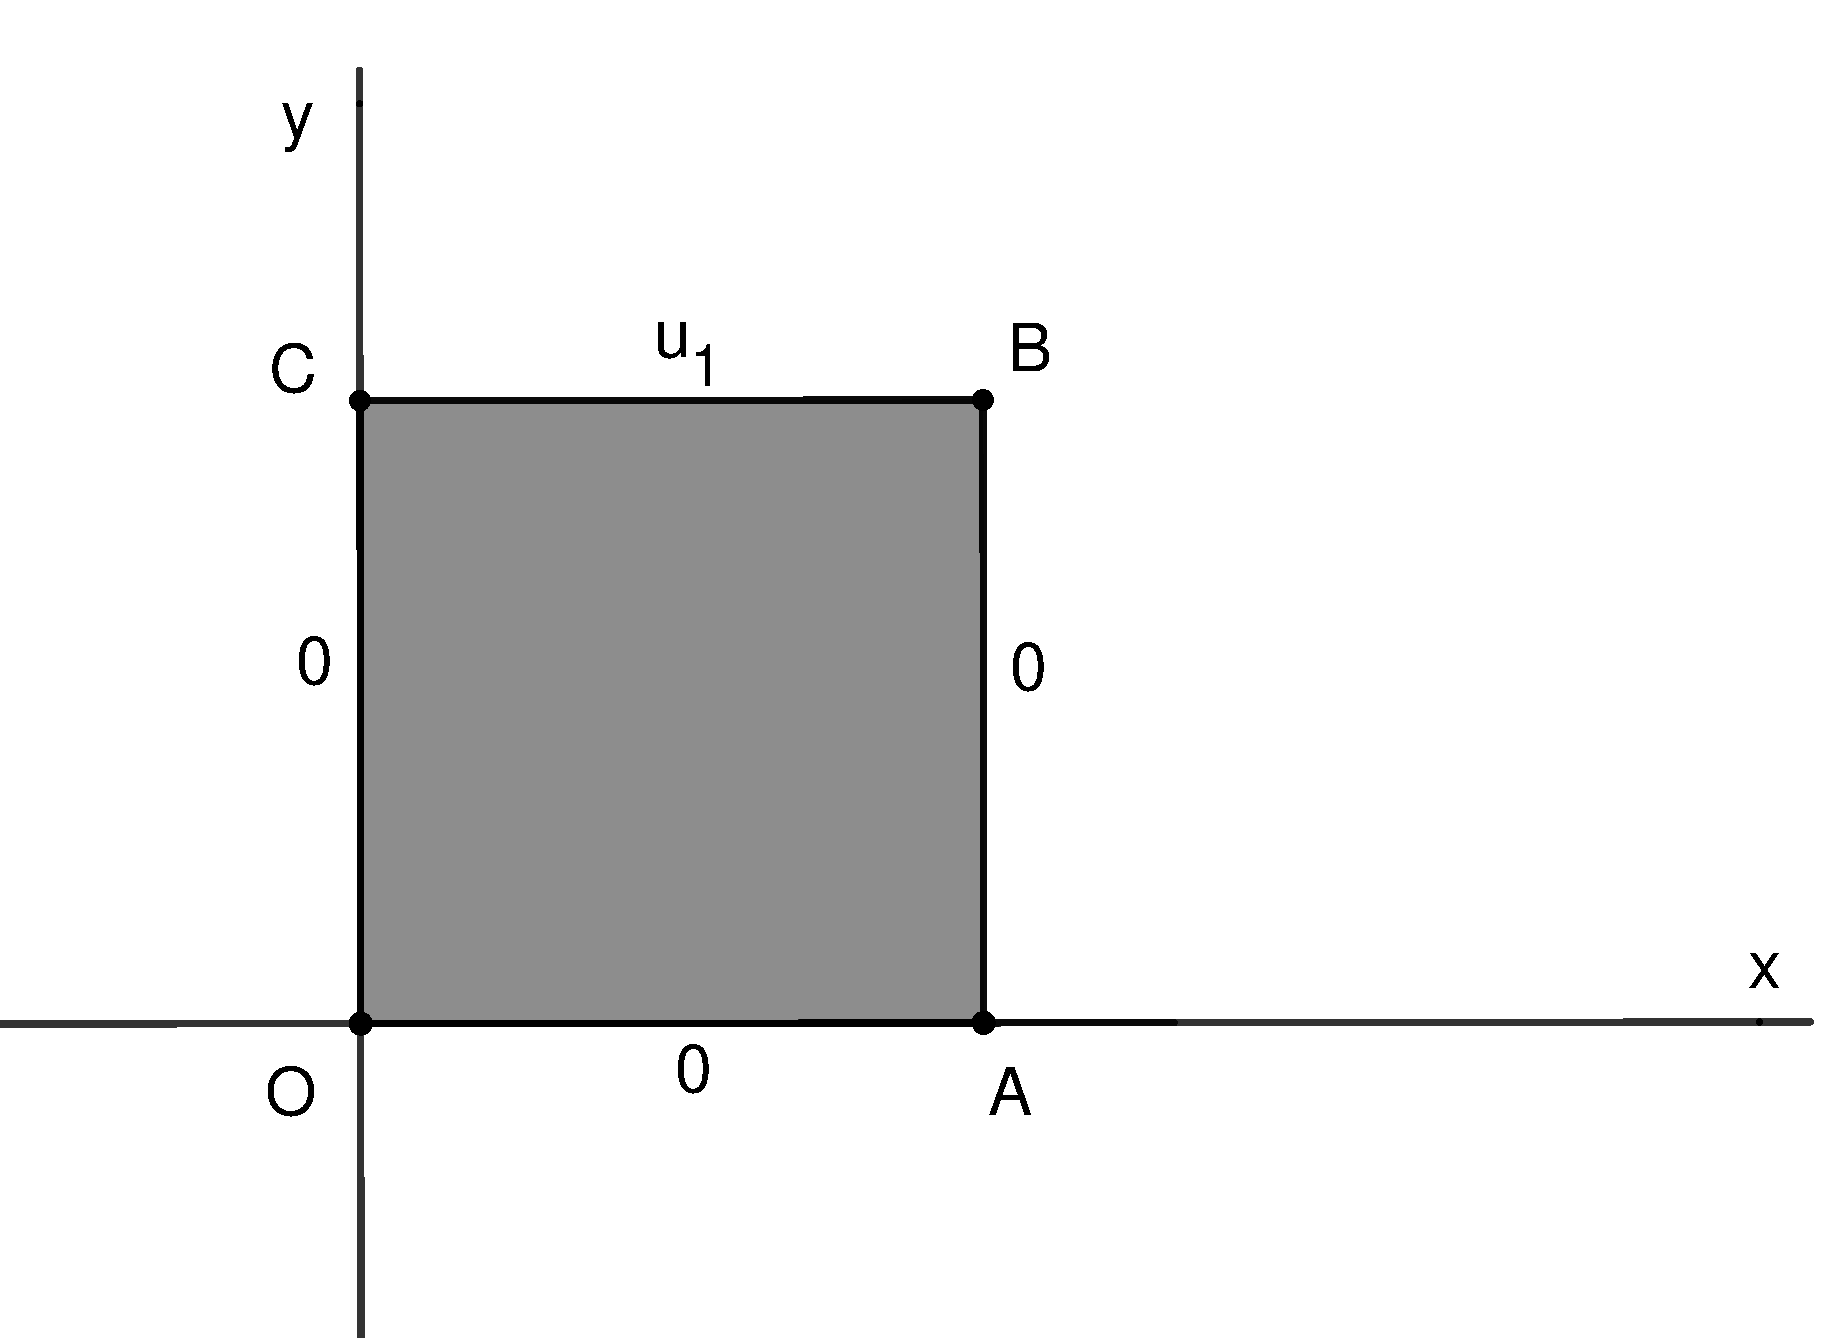
\includegraphics[height=2.5in]{Laplace.pdf} 
\caption{}
\end{figure}

Alegem ca latura care are temperatura $u_1$ s\u a fie cea \^ in care $y=1$, a\c sa cum se poate vedea \^ in Figura 4.1. Deoarece starea de echilibru $u$ nu depinde de timp, vom avea
\begin{equation*}
\frac{\partial u}{\partial t}=0.
\end{equation*}
Ecua\c tia lui Laplace \^ in spa\c tiul bidimensional este
\begin{equation*}
\frac{\partial^2u}{\partial x^2}+\frac{\partial^2u}{\partial y^2}=0.
\end{equation*}
Condi\c tiile de pe frontiera\u a sunt urm\u atoarele:
\begin{equation*}
u(0,y)=u(1,y)=u(x,0)=0,\:  u(x, 1)=u_1 \text{ \c si } \left|u(x,y)\right|<M.
\end{equation*}
Pentru a rezolva aceast\u a problem\u a, vom considera $u=XY$ \c si vom ob\c tine $X''Y+XY''=0$, de unde rezult\u a
\begin{equation}
\frac{X''}{X}=-\frac{Y''}{Y}.
\end{equation}
Fiecare raport din rela\c tia (4.3) reprezint\u a o constant\u a, pe care o vom nota cu $-\lambda^2$. Astfel avem
\begin{equation*}
X''+\lambda^2X=0
\end{equation*}
\c si 
\begin{equation*}
Y''-\lambda^2Y=0, 
\end{equation*}
cu solu\c tiile
\begin{equation*}
X=a_1\cos(\lambda x)+b_1 \sin(\lambda x)
\end{equation*}
\c si 
\begin{equation*}
Y=a_2\cosh(\lambda y)+b_2 \sinh(\lambda y).
\end{equation*}
Deci o posibil\u a solu\c tie este
\begin{equation*}
u(x,y)=\big(a_1\cos(\lambda x)+b_1 \sin(\lambda x)\big)\cdot\big(a_2\cosh(\lambda y)+b_2 \sinh(\lambda y)\big).
\end{equation*}
Din $u(0,y)=0$ rezult\u a $a_1=0$, iar din $u(x, 0)=0$ rezult\u a $a_2=0$. Deci
\begin{equation*}
u(x,y)= b_1\sin(\lambda x)\cdot b_2 \sinh(\lambda y).
\end{equation*}
Din $u(1,y)=0$, rezult\u a $\sin(\lambda)=0$, deci $\lambda =k\pi$, unde $k\in \mathbb{N^*}$. A\c sadar avem
\begin{equation*}
u(x,y)=b_1\sin(k\pi x)\cdot b_2 \sinh(k \pi y)=B\sin(k\pi x)\cdot \sinh(k \pi y).
\end{equation*}
unde B este o constant\u a.
\newline
Utiliz\^ and principiul superpozi\c tiei pentru a satisface ultima condi\c tie, avem
\begin{equation}
u(x,y)=\sum_{k=1}^\infty B_k \sin(k\pi x)\cdot \sinh(k \pi y), 
\end{equation}
apoi din $u(x, 1)=u_1$, ob\c tinem
\begin{equation*}
u_1= \sum_{k=1}^\infty B_k \sin(k\pi x)\sinh(k \pi).
\end{equation*}
Mai departe vom folosi dezvoltarea \^ in serie Fourier pentru a determina coeficien\c tii $B_k$. Consider\u am func\c tia $f(x)=u_1$ pentru $0<x<1$ pe care o vom dezvolta \^ in serie Fourier numai dup\u a sinusuri. Astfel vom extinde definirea lui $f$ la o func\c tie impar\u a pe intervalul (-1, 1), prin periodicitate de perioad\u a 2. Deci avem $L=1$, iar
\begin{equation*}
B_k \sinh(k \pi)=2\int_0^1u_1\sin{k\pi x}\, dx =\frac{2u_1\big(1-cos(\pi x)\big)}{k\pi},
\end{equation*}
de unde rezult\u a
\begin{equation}
B_k=\frac{2u_1\big(1-cos(\pi x)\big)}{k\pi \sinh(k \pi)}.
\end{equation}
Din rela\c tiile (4.4) \c si (4.5), ob\c tinem
\begin{equation*}
u(x,y)=\frac{2u_1}{\pi}\sum_{k=1}^\infty\frac{2u_1\big(1-cos(\pi x)\big)}{k \sinh(k \pi)}\sin(k\pi x)\cdot \sinh(k \pi y).
\end{equation*}
\begin{notice}Aceasta este o problema Dirichlet deoarece am rezolvat ecua\c tia lui Laplace $\nabla^2u=0$, pentru u \^ in interiorul regiunii $R$ considerate, \^ in cazul \^ in care u este specificat a fi pe frontiera regiunii $R$. 
\end{notice}




\subsection*{Aplica\c tie la coarda vibrant\u a}
\paragraph*{}O coard\u a de lungime L este \^ intins\u a \^ intre punctele $(0,0)$ \c si $(L,0)$ de pe axa Ox. La momentul $t=0$, are o form\u a dat\u a de $f(x)$, pentru $0<x<L$, iar \^ in rest este l\u asat\u a liber\u a. Determina\c ti deplasarea coardei \^ in orice moment ulterior. 
\newline
\newline
\textit{Solu\c tie:}
\begin{figure}[H]
\centering
\includegraphics[height=2.5in]{Coarda.pdf} 
\caption{}
\end{figure}
Ecua\c tia coardei vibrante este
\begin{equation*}
\frac{\partial^2y}{\partial t^2}=a^2\frac{\partial^2y}{\partial x^2}, \: 0<x<L, \:t>0,
\end{equation*}
unde $y(x,t)$ este deplasarea coardei fa\c t\u a de axa Ox la momentul t, dup\u a cum se poate vedea \^ in Figura 4.2.
\newline
Capetele coardei se afl\u a \^ in puntele fixe $x=0$ \c si $x=L$ de pe axa Ox, deci
\begin{equation*}
y(0,t)=y(L,t)=0, \: t>0.
\end{equation*} 
Viteza ini\c tial\u a a coardei este zero, 
\begin{equation*}
y_t(x,0)=0,\: 0<x<L.
\end{equation*}
Pentru a rezolva aceast\u a problem\u a, consider\u am $y=XT$. Atunci avem $XT''=a^2X''T $, de unde rezult\u a
\begin{equation}
\frac{T''}{a^2 T}=\frac{X''}{X}.
\end{equation}
Fiecare raport din rela\c tia (4.4) reprezint\u a o constant\u a, pe care o vom nota cu $-\lambda^2$. Astfel avem
\begin{equation*}
X''+\lambda^2X=0
\end{equation*}
\c si 
\begin{equation*}
T''+\lambda^2 a^2 T=0
\end{equation*}
de unde rezult\u a solu\c tiile
\begin{equation*}
X=A_1 \sin(\lambda x)+B_1 \cos(\lambda x)
\end{equation*}
\c si 
\begin{equation*}
T= A_2 \sin(\lambda a t)+B_2 \sin(\lambda a t).
\end{equation*}
Astfel o posibili\u a solu\c tie este dat\u a de
\begin{equation*}
y(x,t)= \big[A_1 \sin(\lambda x)+B_1 \cos(\lambda x)\big] \cdot \big[A_2 \sin(\lambda a t)+B_2 \sin(\lambda a t)\big] 
\end{equation*}
Din $y(0,t)=0$, rezult\u a $B_1=0$ \c si 
\begin{equation*}
y(x,t)= A_1 \sin(\lambda x)\cdot \big[A_2 \sin(\lambda a t)+B_2 \sin(\lambda a t)\big]= \sin(\lambda x)\big[A \sin(\lambda a t)+B \sin(\lambda a t)\big]
\end{equation*}
\c si 
\begin{equation*}
y_t(x,yt)=\sin(\lambda x)\big[ A\lambda a\cos(\lambda at)-B\lambda a \sin(\lambda at) \big],
\end{equation*}
unde A, B sunt constante. 
\newline
Din $y(L,t)=0$, avem 
\begin{equation*}
y(L,t)=\sin(\lambda L)\big[A \sin(\lambda a t)+B \sin(\lambda a t)\big] =0, 
\end{equation*}
de unde rezult\u a $\sin(\lambda L)=0$, pentru c\u a cel de-al doilea factor nu poate fi zero, deci $\lambda=\frac{k\pi}{L},\: k\in \mathbb{Z}$. Din $y_t(x,0)=0$, rezult\u a
\begin{equation*}
A\lambda a\sin(\lambda x)=0.
\end{equation*}
Deci $A=0$, pentru c\u a factorul cu sinus nu poate fi 0. Astfel avem
\begin{equation*}
y(x,t)=B\sin\Big(\frac{k\pi x}{L}\Big)\cos\Big(\frac{k \pi a t}{L}\Big).
\end{equation*}
Pentru a satisface condi\c tia $y(x,0)=f(x)$, este necesar s\u a apel\u am la principiul superpozi\c tiei, deci
\begin{equation*}
y(x,t)=\sum_{k=1}^\infty\sin\Big(\frac{k\pi x}{L}\Big)\cos\Big(\frac{k \pi a t}{L}\Big).
\end{equation*}
Din condi\c tia $y(x,0)=f(x)$, ob\c tinem
\begin{equation*}
f(x)=\sum_{k=1}^\infty\sin\Big(\frac{k\pi x}{L}\Big).
\end{equation*}
\c Tin\^ and cont de coeficien\c tii dezvolt\u arii \^ in serie Fourier a func\c tiei $f(x)$, pentru $x\in (0,L)$, ob\c tinem
\begin{equation*}
B_k=\frac{2}{L}\int_0^L f(x)\sin\Big(\frac{k\pi x}{L}\Big)\, dx.
\end{equation*}
Astfel ajungem la solu\c tia
\begin{equation*}
y(x,t)=\sum_{k=1}^\infty \frac{2}{L}\int_0^L f(x)\sin\Big(\frac{k\pi x}{L}\Big)\, dx\sin\Big(\frac{k\pi x}{L}\Big)\cos\Big(\frac{k \pi a t}{L}\Big).
\end{equation*}







\addcontentsline{toc}{chapter}{Bibliografie}
\begin{thebibliography}\\
\bibitem{}FIHTENHOL\c T G.M., \textit{Curs de calcul diferen\c tial \c si integral}, Editura Tehnic\u a, Bucure\c sti 1965.
\bibitem{}MUNTEAN I. \textit{Analiz\u a func\c tional\u a}, Cluj-Napoca, 1993.
\bibitem{}MURRAY R. SPIEGEL, \textit{Theory and problems of Fourier Analysis with applications to Boundary value problems}, Schaum's Outline Series, McGraw-Hill Book Company.
\bibitem{}PETER L. DUREN, \textit{Invitation to Classical Analysis}, Volumul 17 din \textit{Pure and applied undergraduate texts, The Sally series}, Editura American Mathematical Society, 2012.
\bibitem{}SOLOMON M., MIRON N., \textit{Analiz\u a matematic\u a, volumul II}, Editura Didactic\u a \c si Pedagogic\u a.
\bibitem{}WREDE R., MURRAY R. SPIEGEL, \textit{Advenced Calculus}, a treia edi\c tie, Schaum's Outline Series, McGraw-Hill Companies.

\bibitem{}$civile.utcb.ro/cmat/cursrt/ec1.pdf$.
\bibitem{}$www.utgjiu.ro/math/miovanov/book/ms\_curs/cap4.pdf$.
\bibitem{}$https://en.wikipedia.org/wiki/Fourier\_series$.
\bibitem{}$https://ro.wikipedia.org/wiki/Serie\_Fourier$.
\end{thebibliography}
\end{document}